\chapter{راهنمای استفاده}

در این فصل راهنمای مورد نیاز برای کاربران آرنو آورده شده است.
در کنار این راهنما، در رابط کاربری هم گزینه‌ای برای مشاهده‌ی راهنمای‌ها در نظر گرفته شده که با توجه به عدم دسترسی کاربران عادی به این مستند می‌تواند مفید باشد.

پس از باز کردن آرنو صفحه‌ی \ref{home} نمایش داده می‌شود و همه‌ی کاربران برای استفاده از آرنو باید از طریق صفحه‌ی \ref{login} وارد سایت شوند. 

\begin{figure}[h]
	\centering
	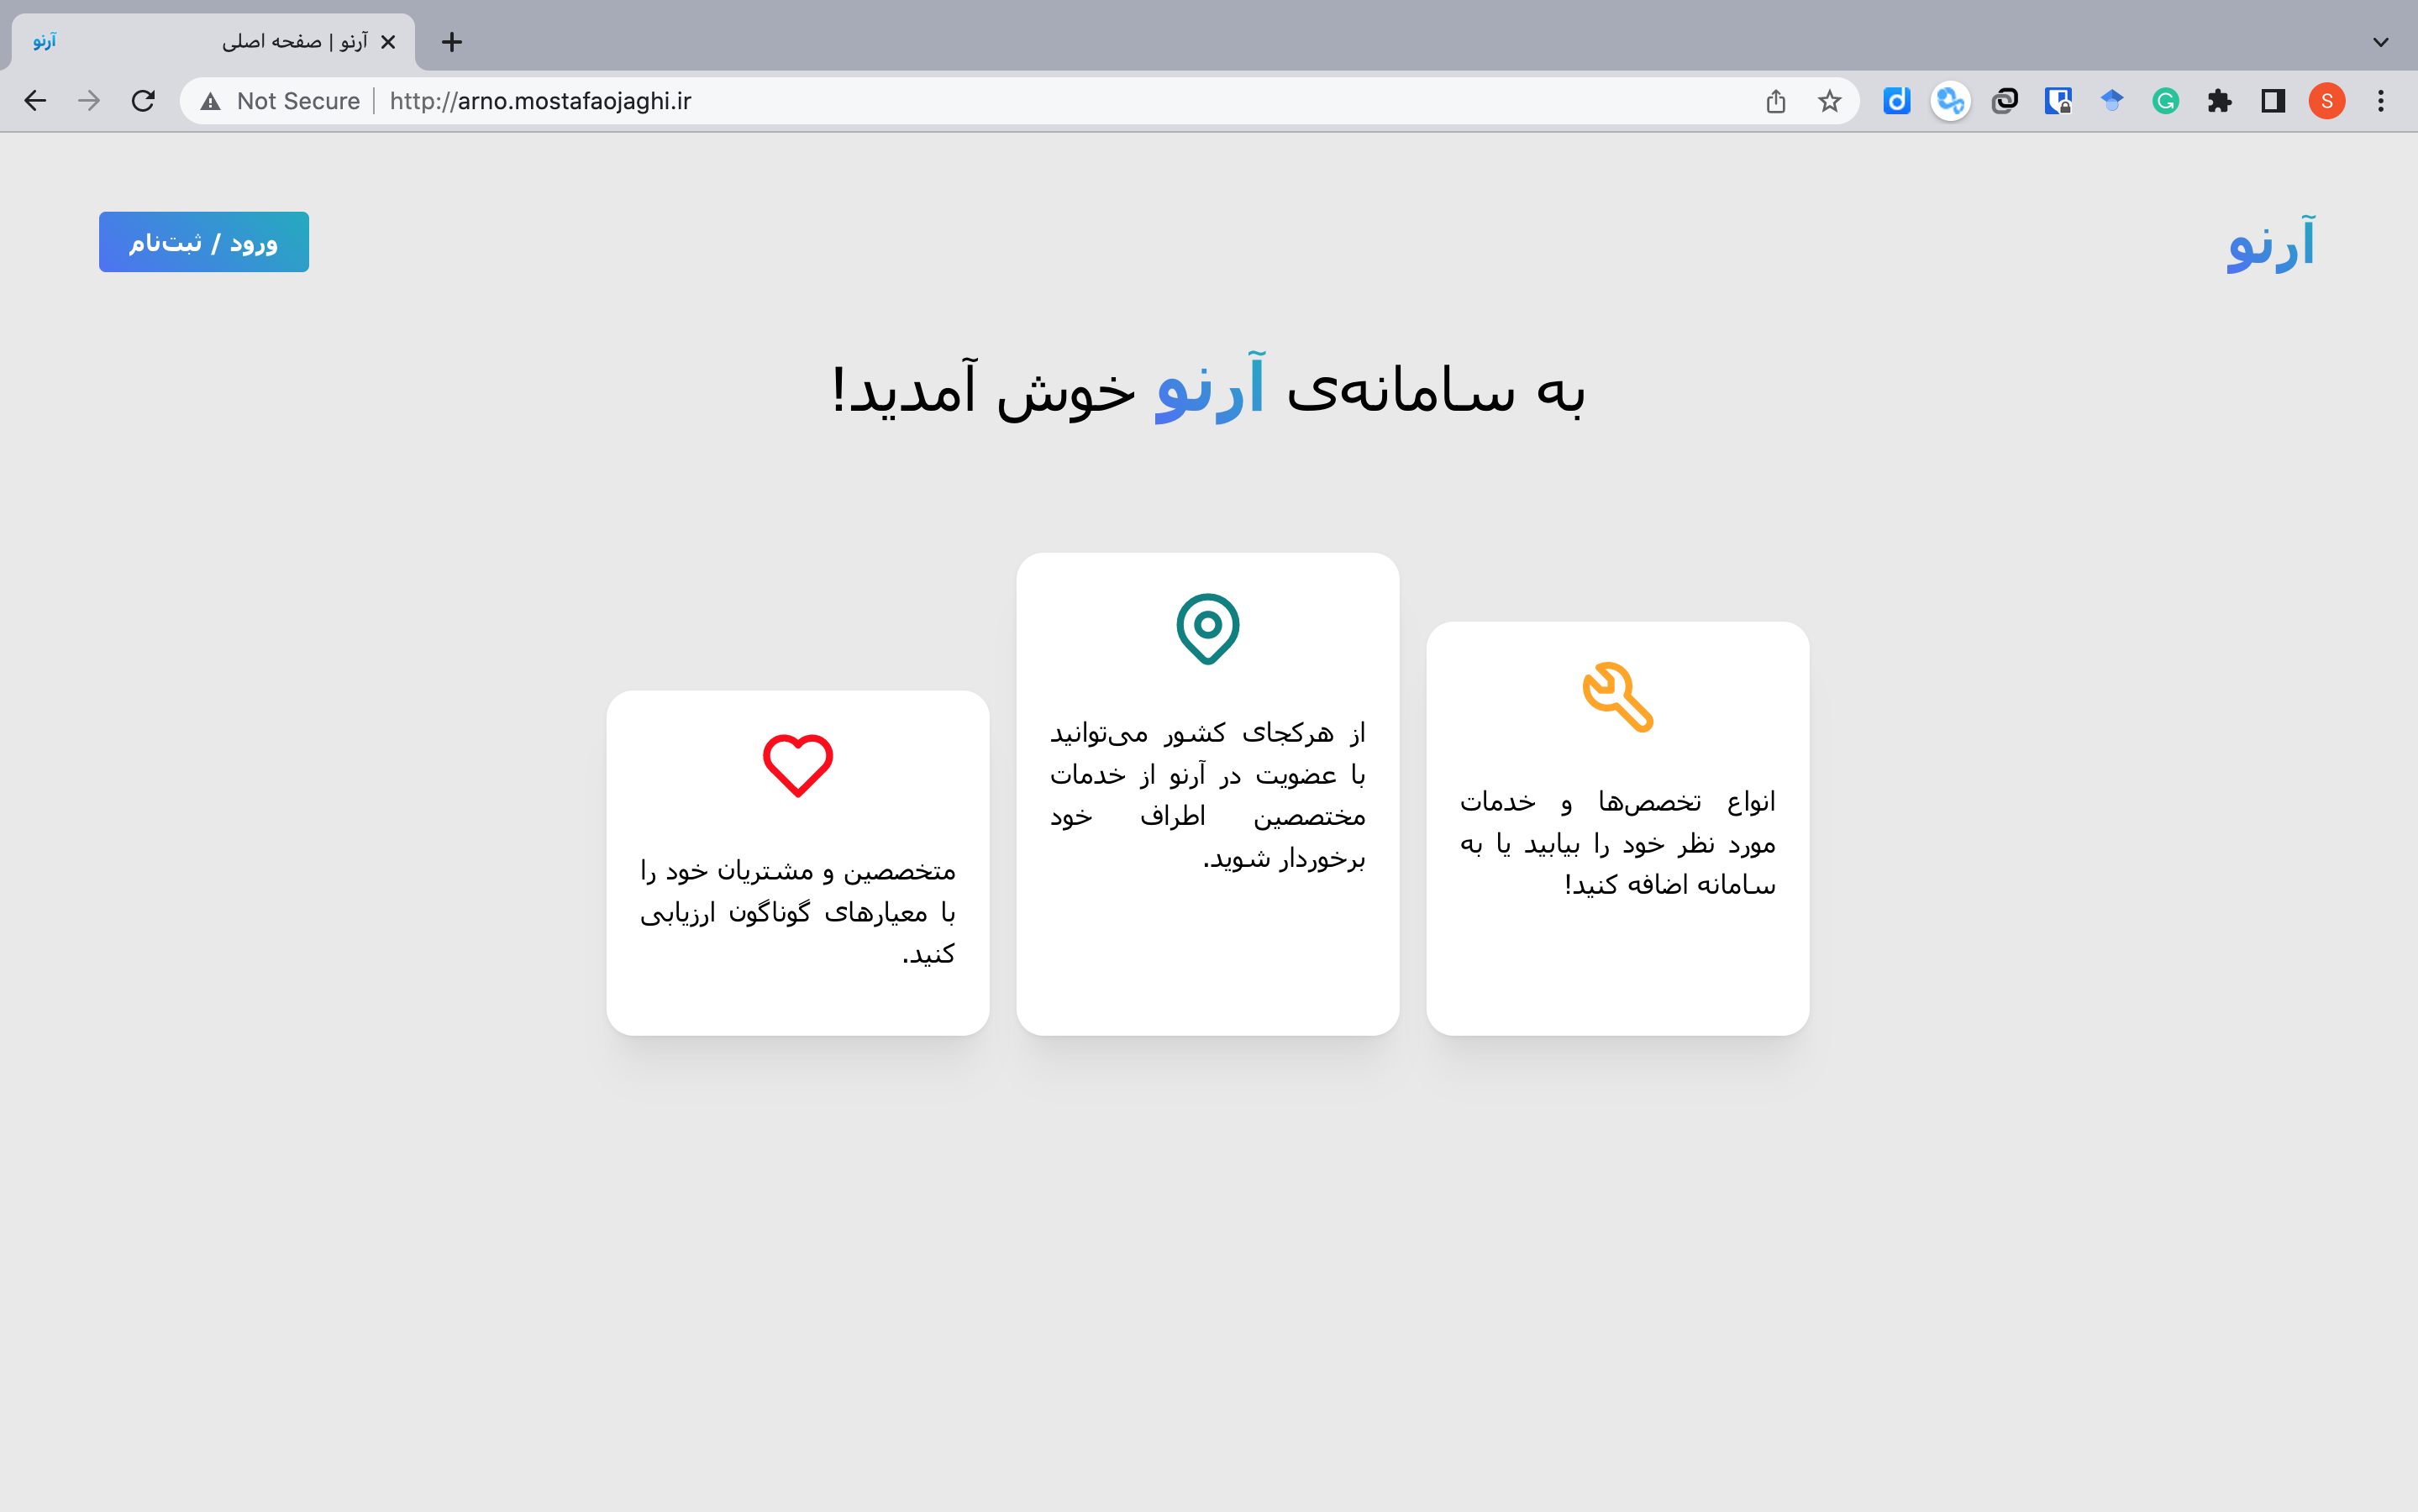
\includegraphics[width=\textwidth]{figs/user-guide/home}
	\caption{صفحه اصلی}
	\label{home}
\end{figure}

\begin{figure}[h]
	\centering
	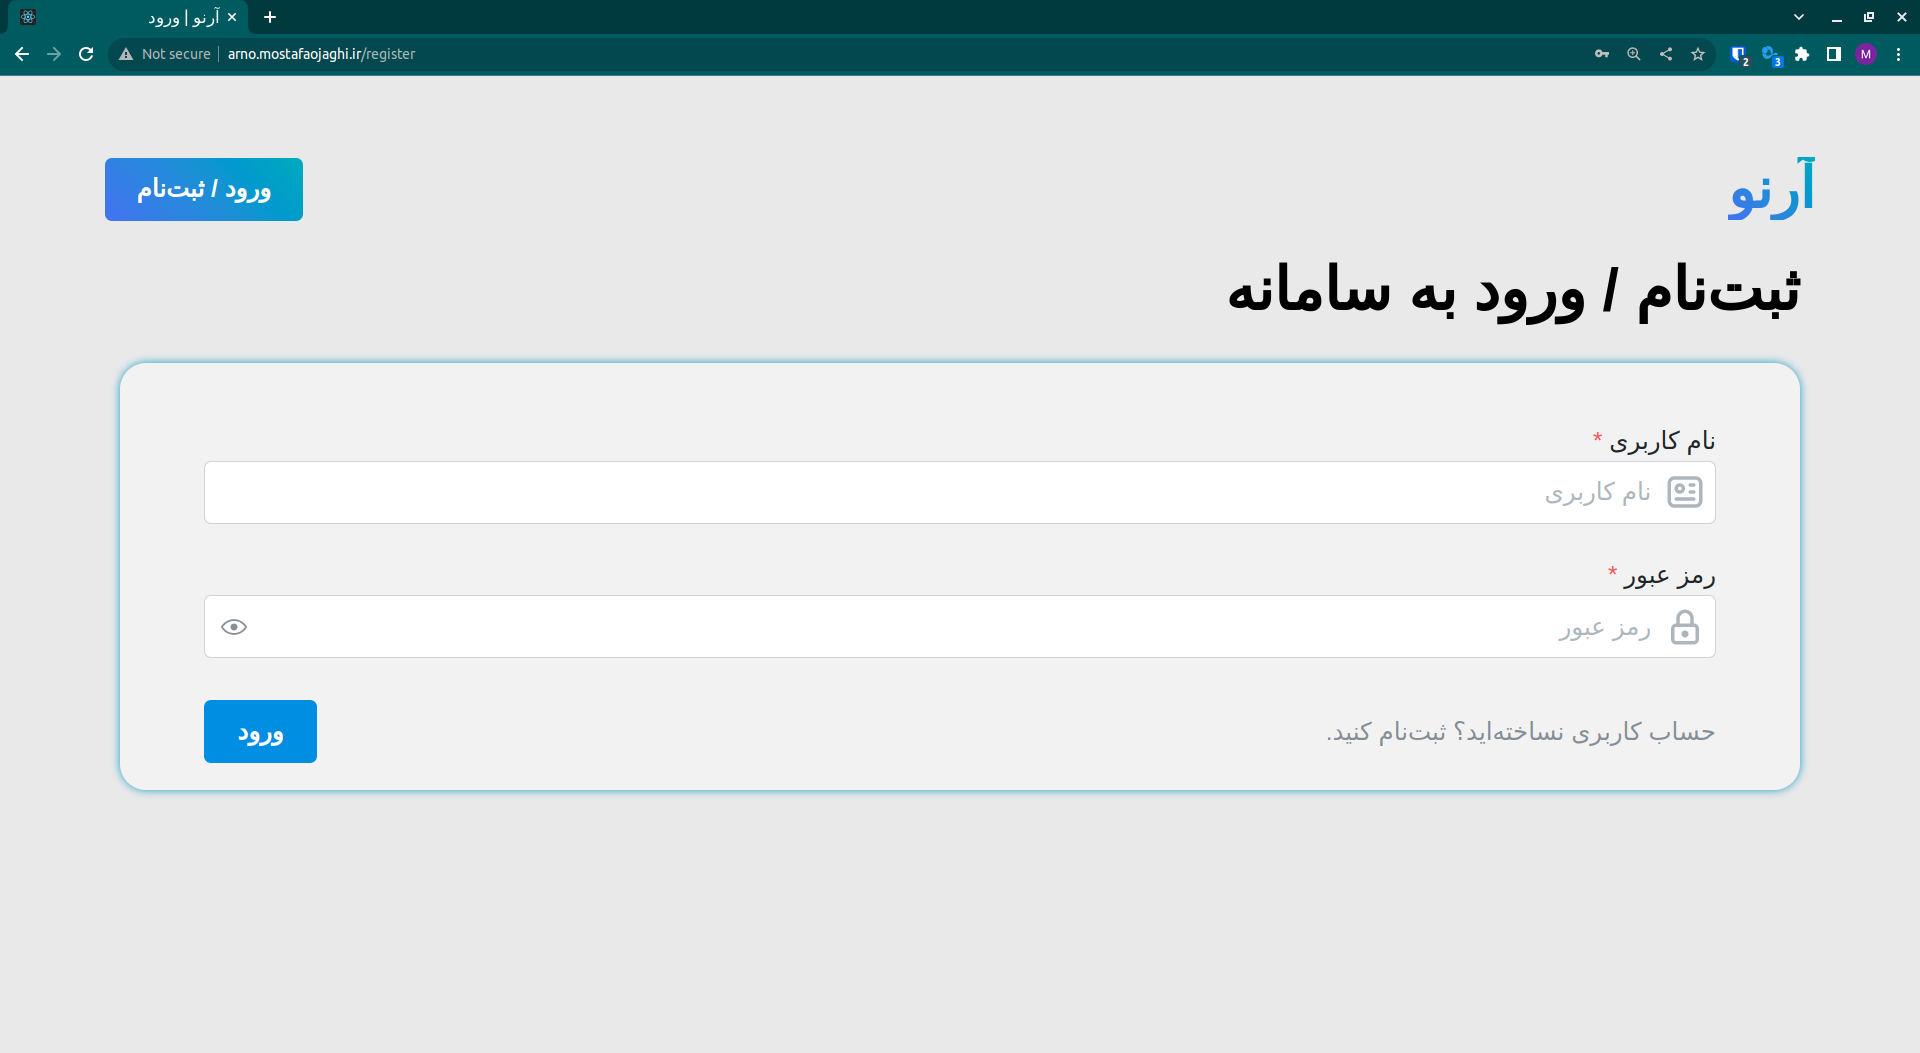
\includegraphics[width=\textwidth]{figs/user-guide/login}
	\caption{صفحه ورود}
	\label{login}
\end{figure}

در ادامه راهنمای لازم برای هر یک از انواع کاربران آورده ‌شده است.

\FloatBarrier
\section{راهنمای مشتریان}

برای استفاده از خدمات سایت به عنوان مشتری ابتدا باید در سایت ثبت‌نام کنید. برای این کار در قسمت پایینی صفحه‌ی \ref{login} روی گزینه‌ی ثبت‌نام کلیک کنید.
با این کار وارد صفحه‌ی \ref{customer-signup} می‌شوید. پس از وارد کردن اطلاعات مورد نیاز بر روی گزینه‌ی ثبت‌نام کلیک کنید.
در صورت صحت اطلاعات وارد شده حساب کاربری شما ساخته می‌شود و به صورت خودکار وارد سایت می‌شوید.
در غیر این صورت از شما خواسته می‌شود که اطلاعات خود را اصلاح کنید.

\begin{figure}[h]
	\centering
	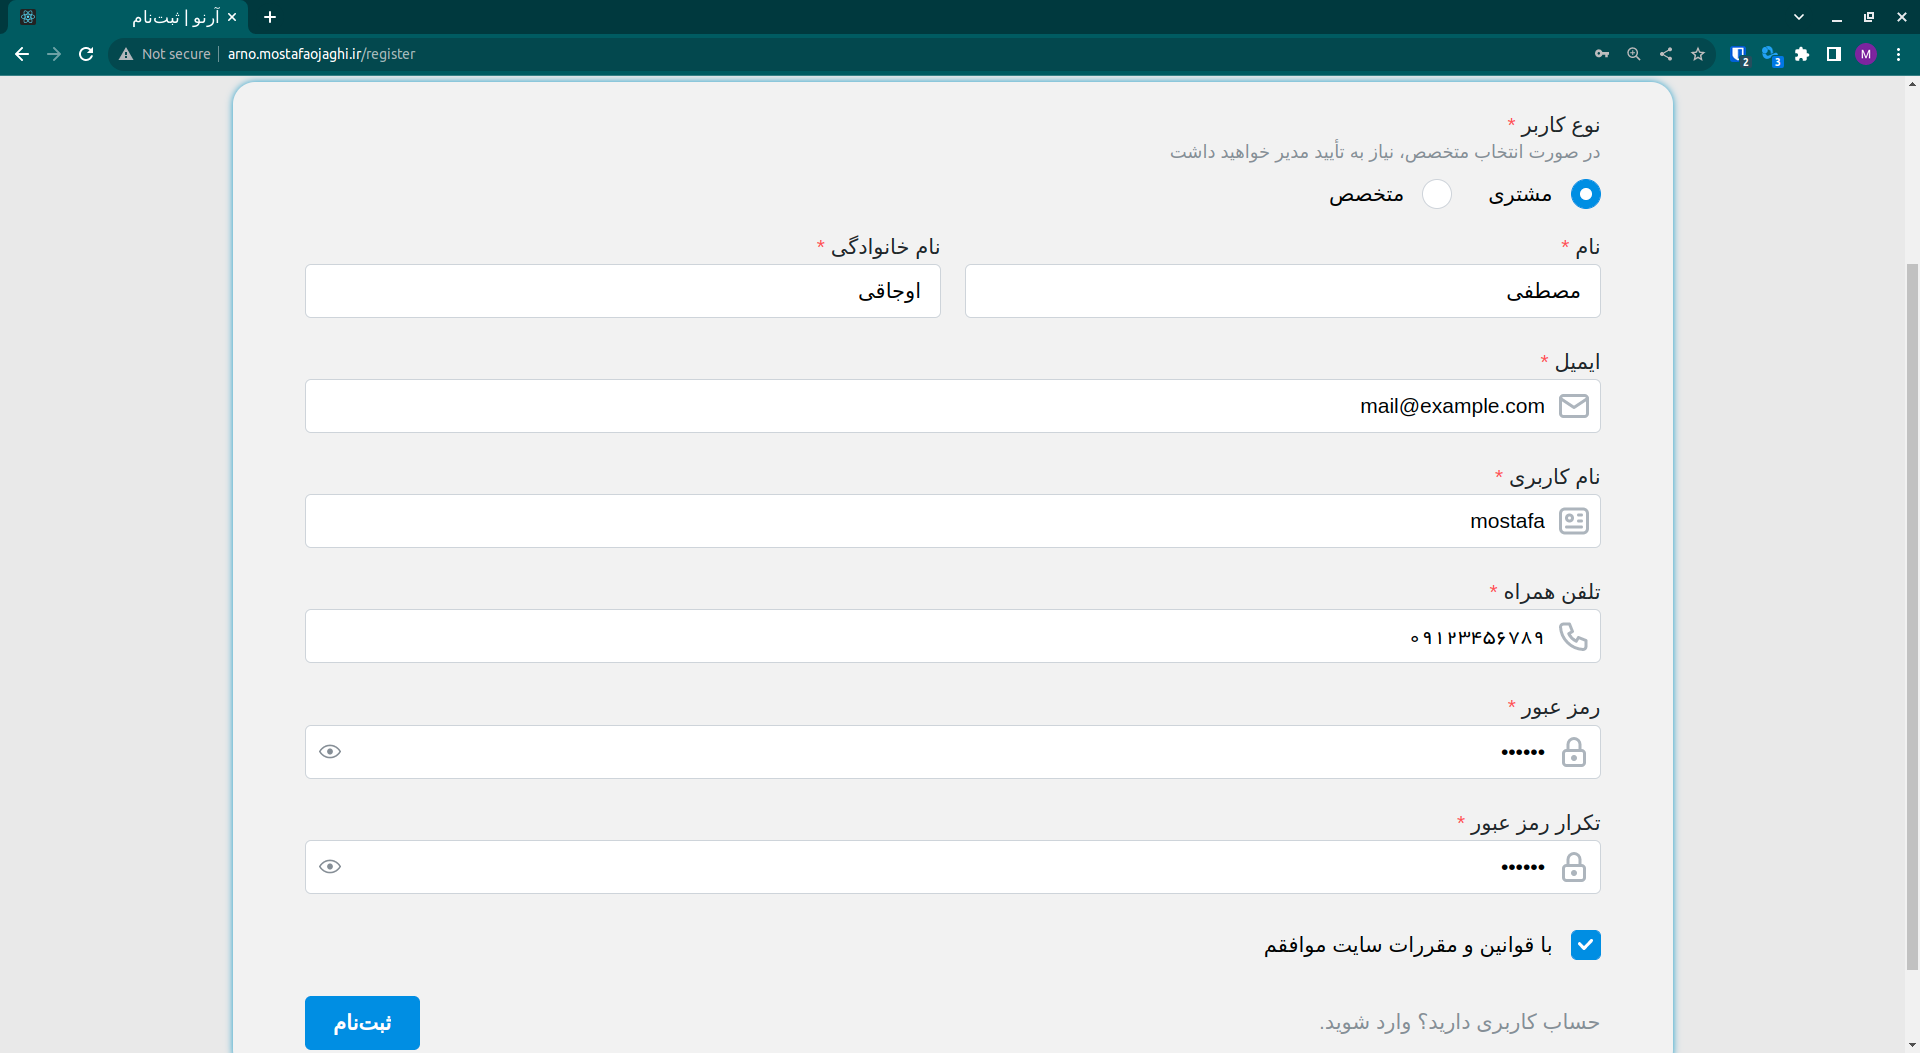
\includegraphics[width=\textwidth]{figs/user-guide/customer-signup}
	\caption{صفحه ثبت‌نام مشتری}
	\label{customer-signup}
\end{figure}

پس از ورود به سیستم صفحه‌ی \ref{customer-dashboard} به شما نمایش داده می‌شود.
در سمت راست این صفحه لینک‌هایی به قسمت‌های مختلف سامانه و در گوشه‌ی سمت چپ و بالای آن دکمه‌های اعلان‌ها، راهنما و خروج از سامانه قرار دارد.

\begin{figure}[h]
	\centering
	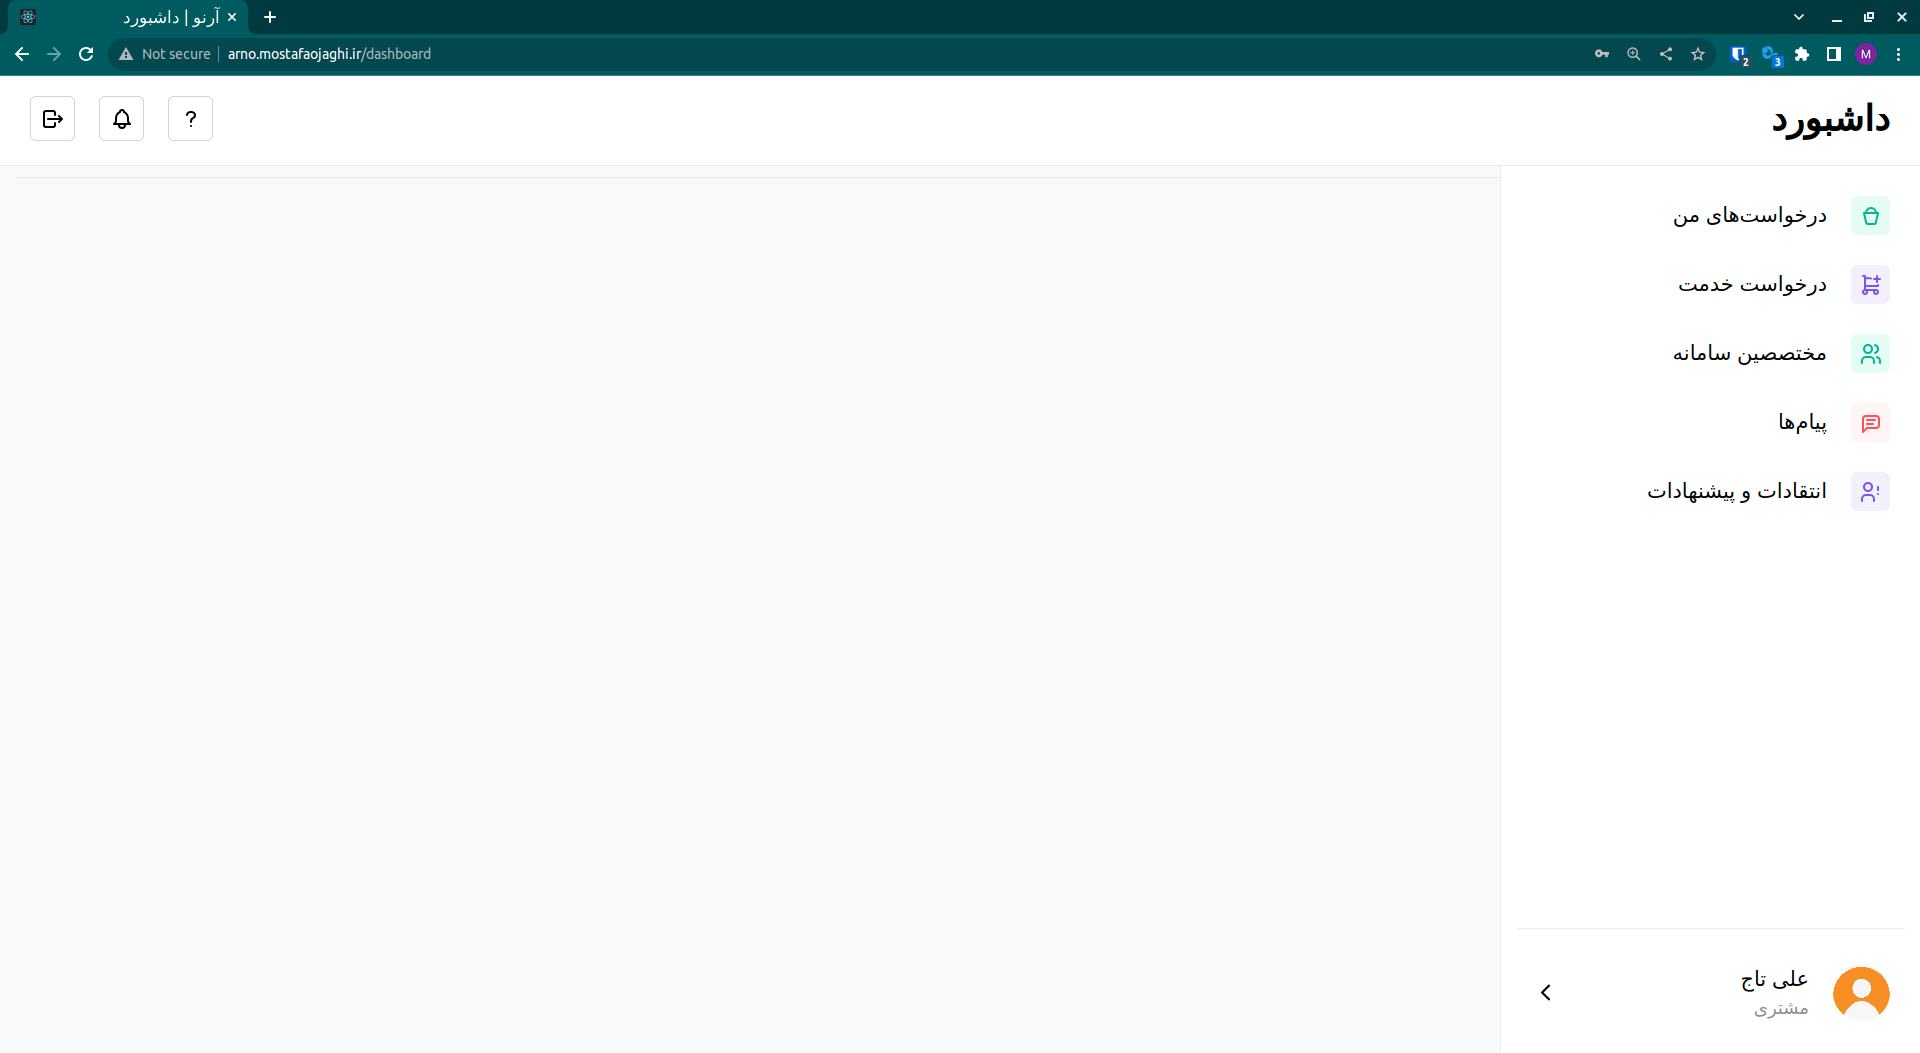
\includegraphics[width=\textwidth]{figs/user-guide/customer-dashboard}
	\caption{صفحه اصلی مشتری}
	\label{customer-dashboard}
\end{figure}

برای ثبت درخواست خود باید به منوی درخواست خدمت مراجعه کنید.
در این صفحه مطابق شکل \ref{customer-request} نوع خدمت مورد نیاز و تاریخ شروع آن را مشخص می‌کنید.
سپس آدرس انجام خدمت و توضیحات خدمت خواسته شده را مشخص کرده و سفارش را ثبت می‌کنید.
پس از ثبت سفارش برای پیگیری آن باید به منوی «درخواست‌های من» مراجعه کنید.
در این صفحه می‌توانید وضعیت و جزییات درخواست خود را مشاهده کرده و اقدامات لازم را در مورد آن‌ها انجام دهید.

\begin{figure}[h]
	\centering
	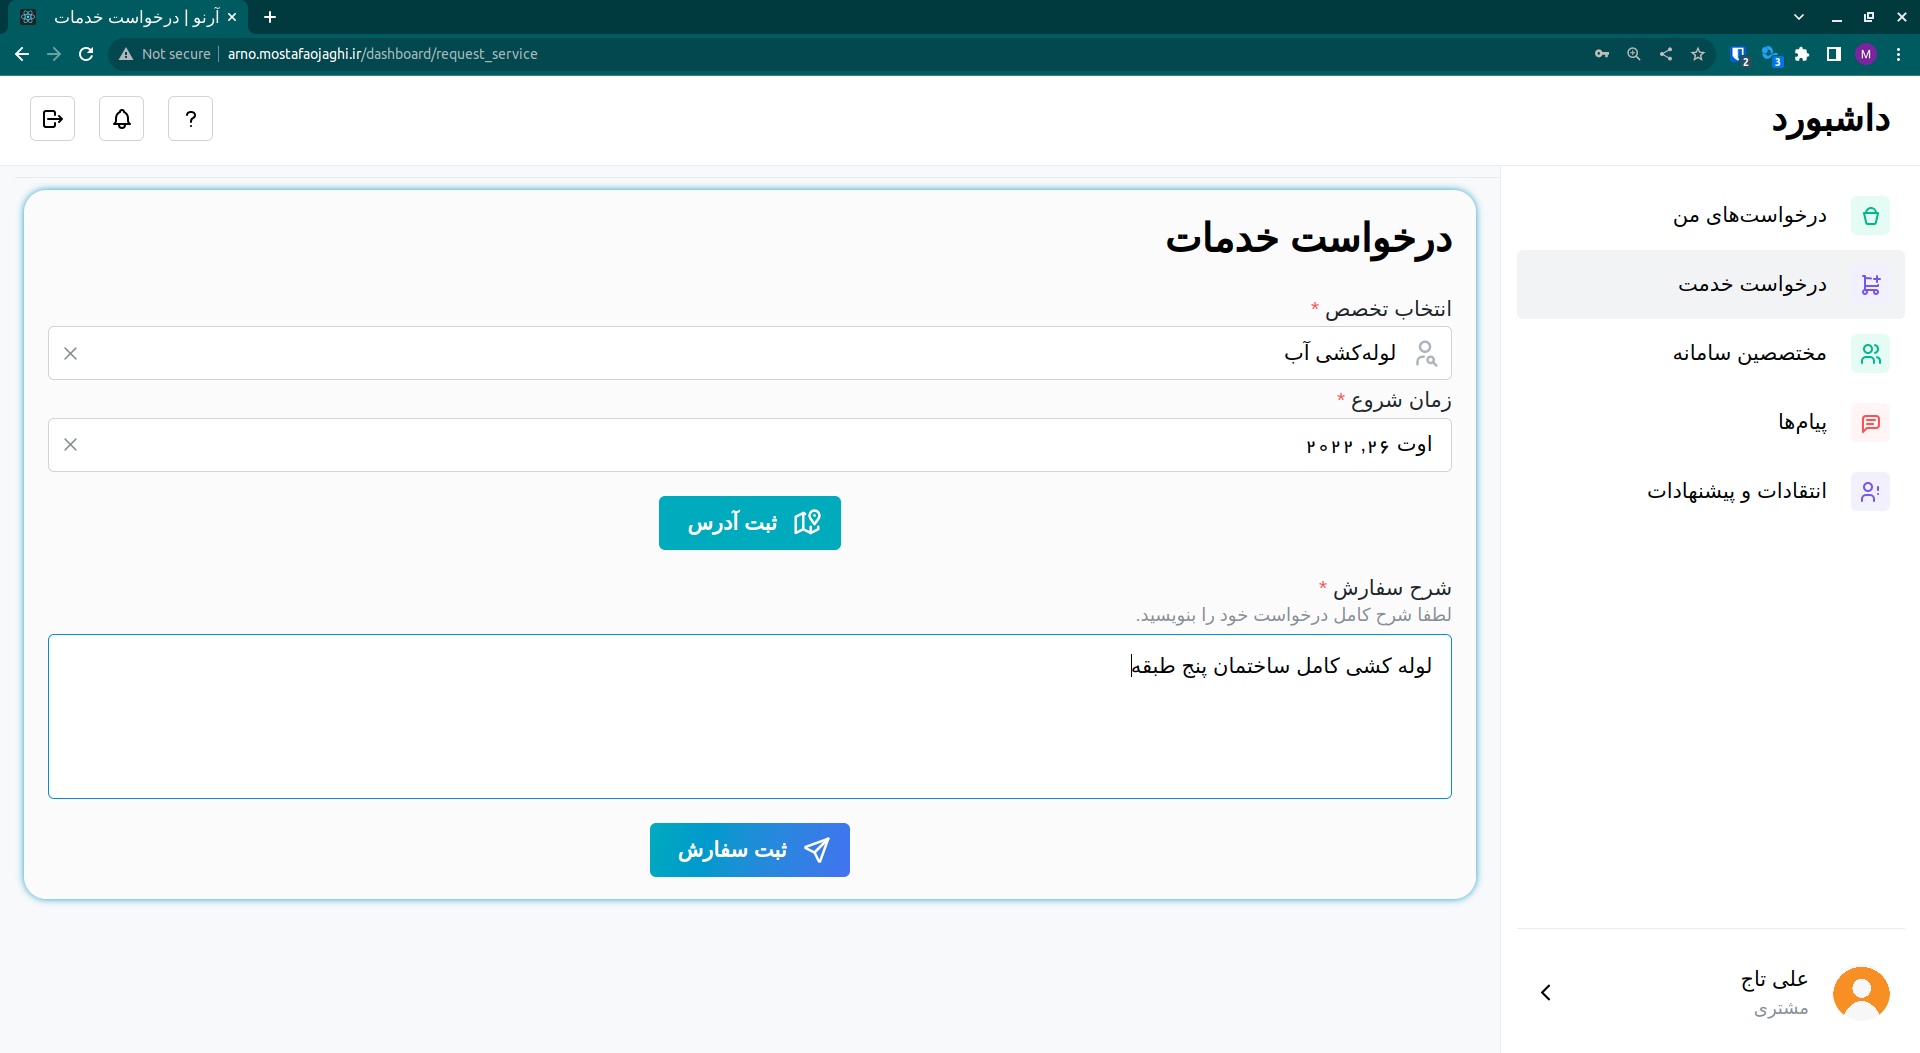
\includegraphics[width=\textwidth]{figs/user-guide/customer-request}
	\caption{صفحه درخواست خدمت}
	\label{customer-request}
\end{figure}

منوی انتقادات و پیشنهادات (شکل \ref{customer-technical-feedback}) برای ثبت انتقادات و پیشنهادات و همچنین ثبت مشکلات فنی سامانه طراحی شده است.
از این طریق می‌توانید مشکلات و نظرات خود را به گوش مدیران شرکت برسانید.

\begin{figure}[h]
	\centering
	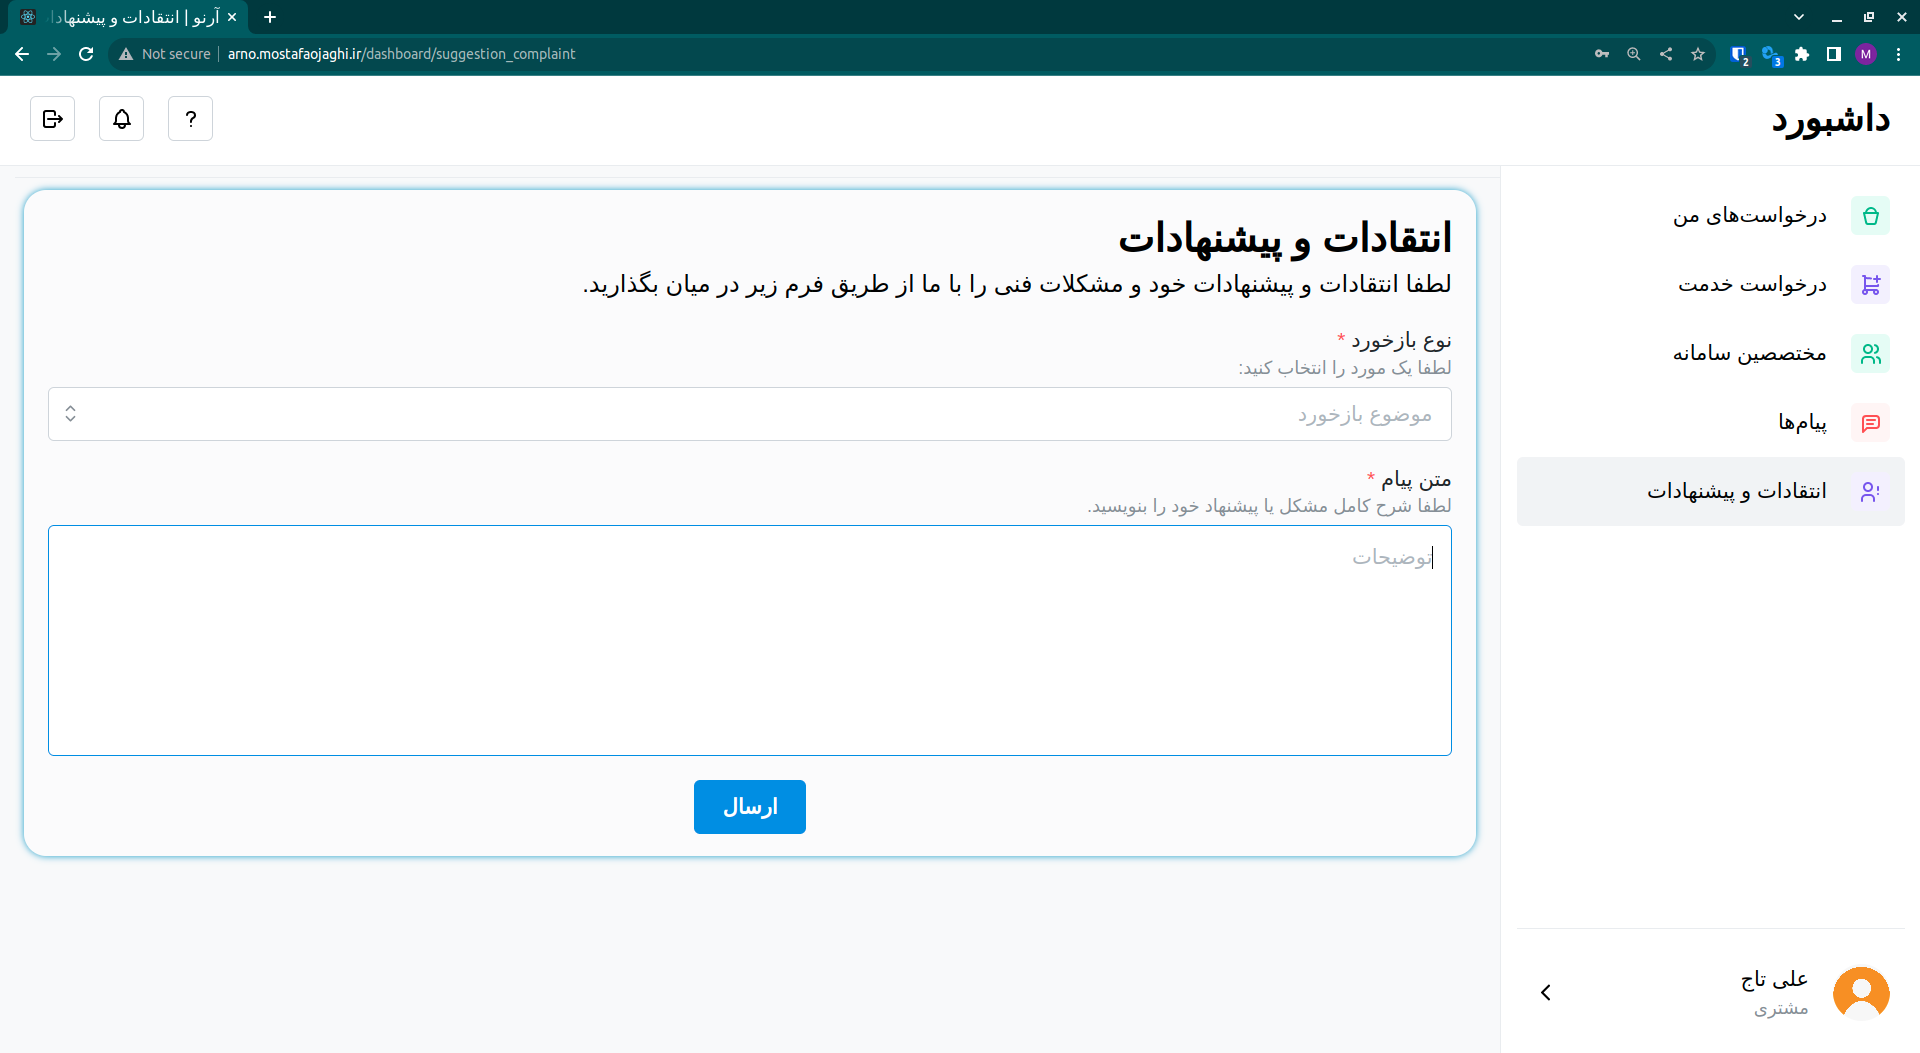
\includegraphics[width=\textwidth]{figs/user-guide/customer-technical-feedback}
	\caption{صفحه انتقادات و پیشنهادات}
	\label{customer-technical-feedback}
\end{figure}



\FloatBarrier
\section{راهنمای متخصصان}

برای استفاده از سایت به عنوان متخصص هم ابتدا باید در سایت ثبت‌نام کنید.
برای ثبت نام متخصص علاوه بر اطلاعات مورد نیاز در ثبت‌نام مشتری، باید تعدادی تخصص را که مایلید در آن‌ها فعالیت کنید، مشخص کنید.
صفحه‌ی ثبت‌نام متخصصان در شکل \ref{specialist-signup} نشان داده شده است.
در صورت موفقیت آمیز بودن ثبت‌نام به صفحه‌ی اصلی (شکل \ref{specialist-dashboard}) هدایت می‌شوید.

\begin{figure}[h]
	\centering
	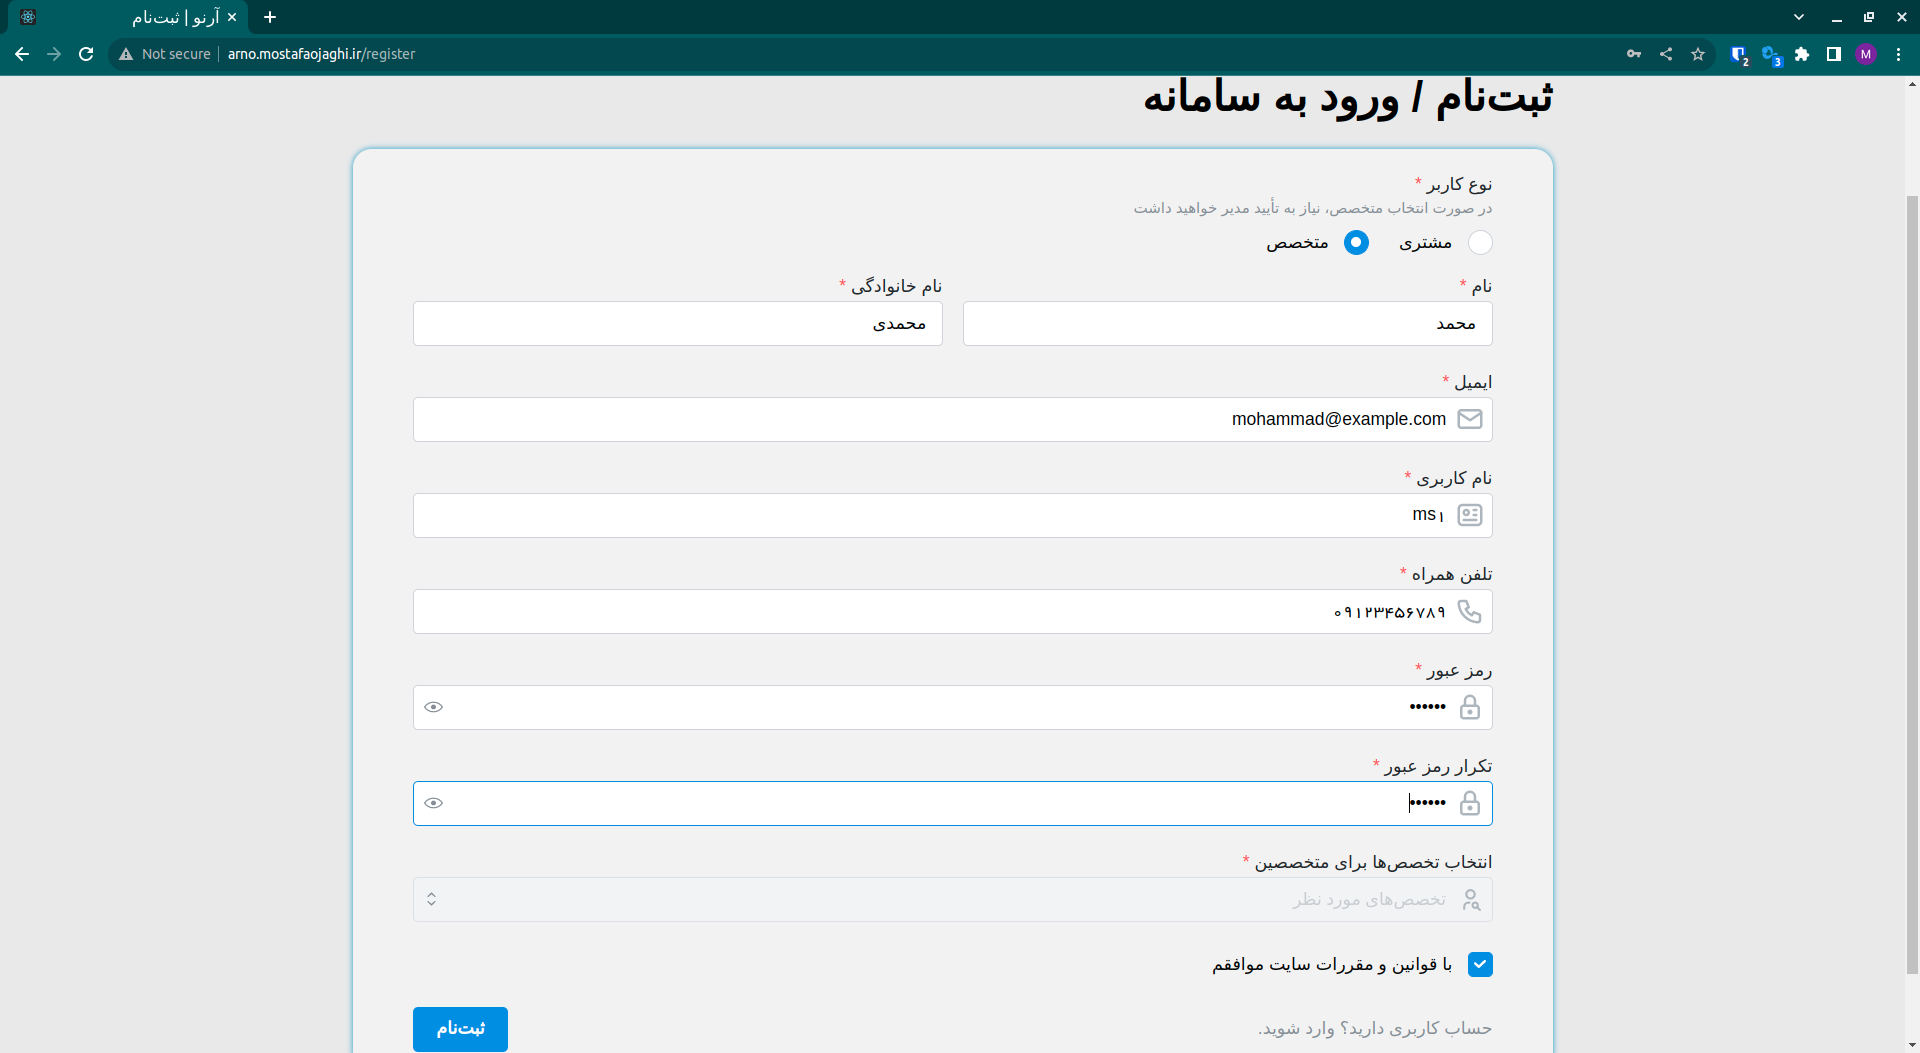
\includegraphics[width=\textwidth]{figs/user-guide/specialist-signup}
	\caption{صفحه ثبت‌نام متخصص}
	\label{specialist-signup}
\end{figure}

\begin{figure}[h]
	\centering
	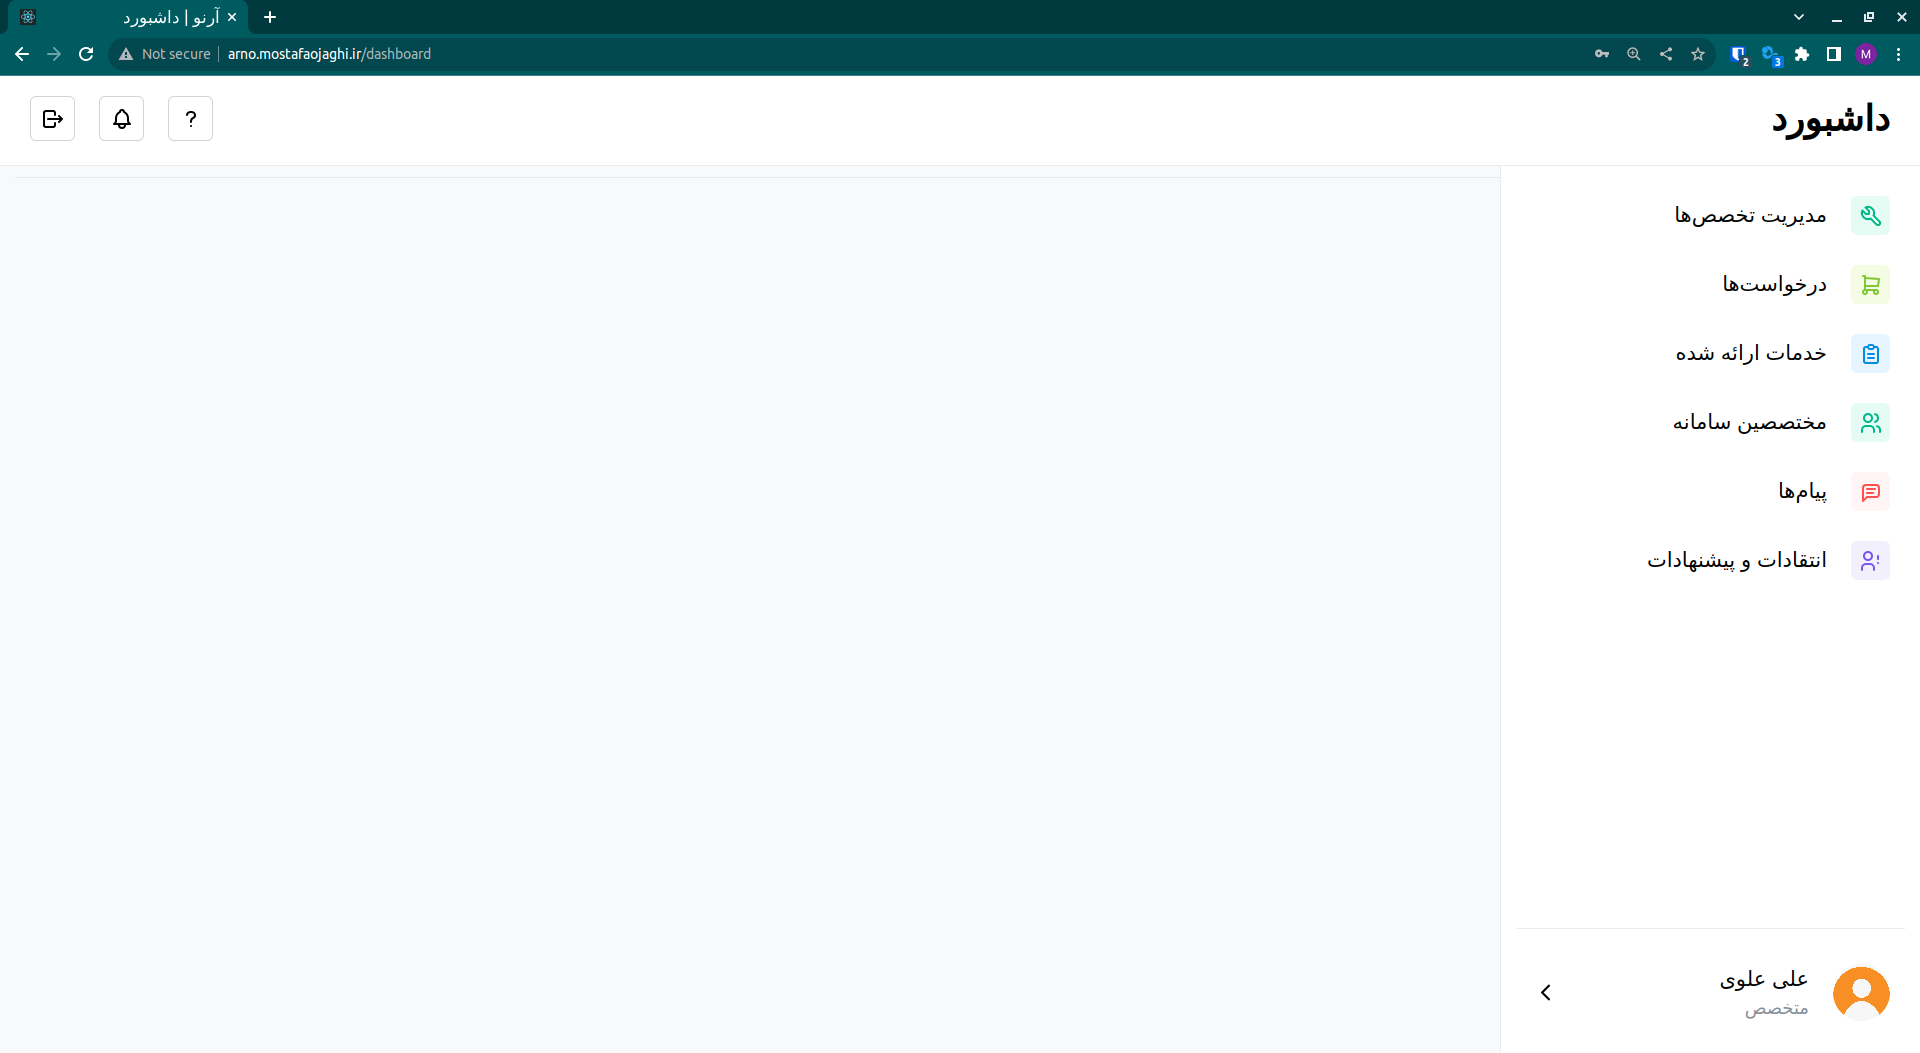
\includegraphics[width=\textwidth]{figs/user-guide/specialist-dashboard}
	\caption{صفحه ثبت‌نام متخصص}
	\label{specialist-dashboard}
\end{figure}

\FloatBarrier
خدمات آرنو در تخصص‌هایی مشخص انجام می‌شود که در دسته‌های کلی‌تری برای کاربری بهتر قرار می‌گیرند.
شما با استفاده از منوی مدیریت تخصص‌ها (شکل \ref{specialist-manage-specialities})  می‌توانید این دسته‌ها و تخصص‌ها را مشاهده کرده، تخصص‌های جدیدی به آن‌ها بیافزایید.
برای افزودن تخصص در مطابق شکل \ref{specialist-add-speciality} باید نام تخصص مورد نظر، دسته‌بندی آن و توضیحات لازم را اضافه کنید و دکمه‌ی ایجاد تخصص را بفشارید.
پس از افزودن تخصص مورد نظر خود به سامانه می‌توانید با ویرایش پروفایل خود (شکل \ref{specialist-profile}) این تخصص را به تخصص‌های خود بیافزایید.
همچنین در این منو امکان حذف یک تخصص و غیر فعال کردن ارائه‌ی سرویس وجود دارد.

\begin{figure}[h]
	\centering
	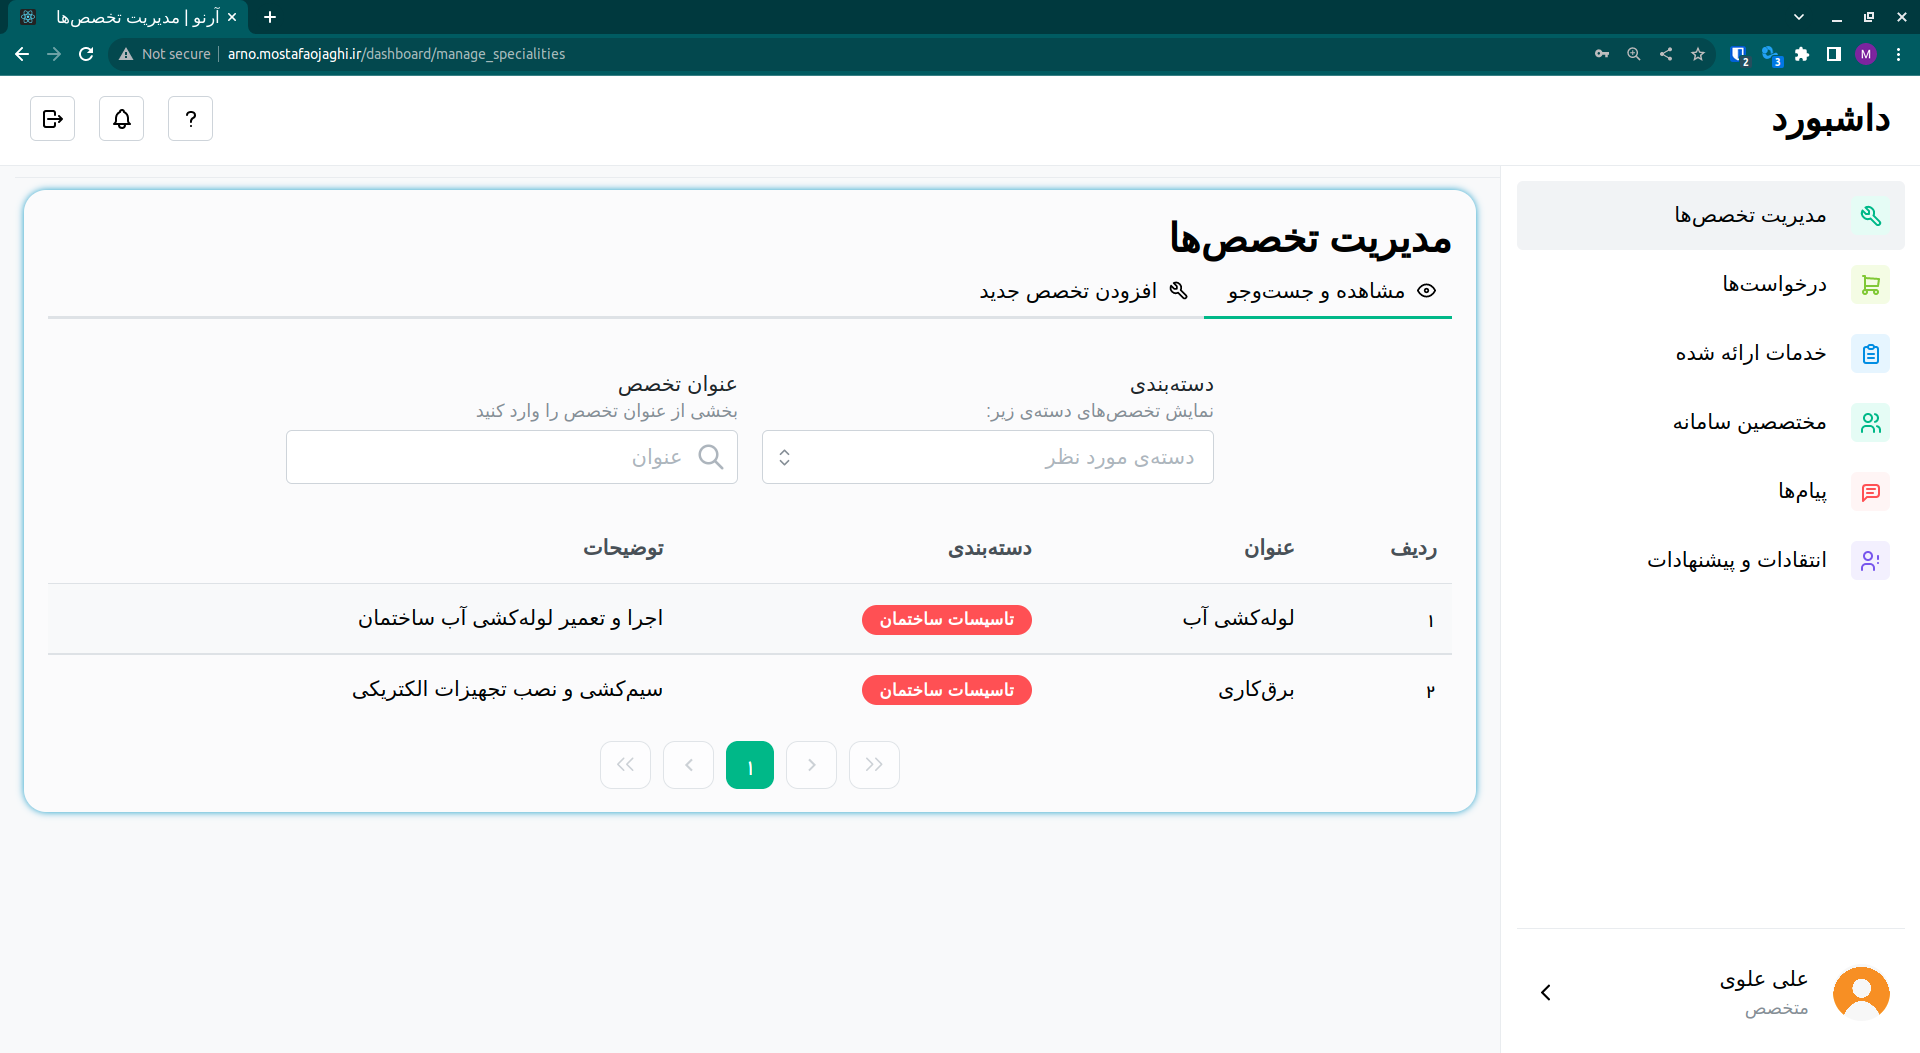
\includegraphics[width=\textwidth]{figs/user-guide/specialist-manage-specialities}
	\caption{صفحه مدیریت تخصص‌ها}
	\label{specialist-manage-specialities}
\end{figure}

\begin{figure}[h]
	\centering
	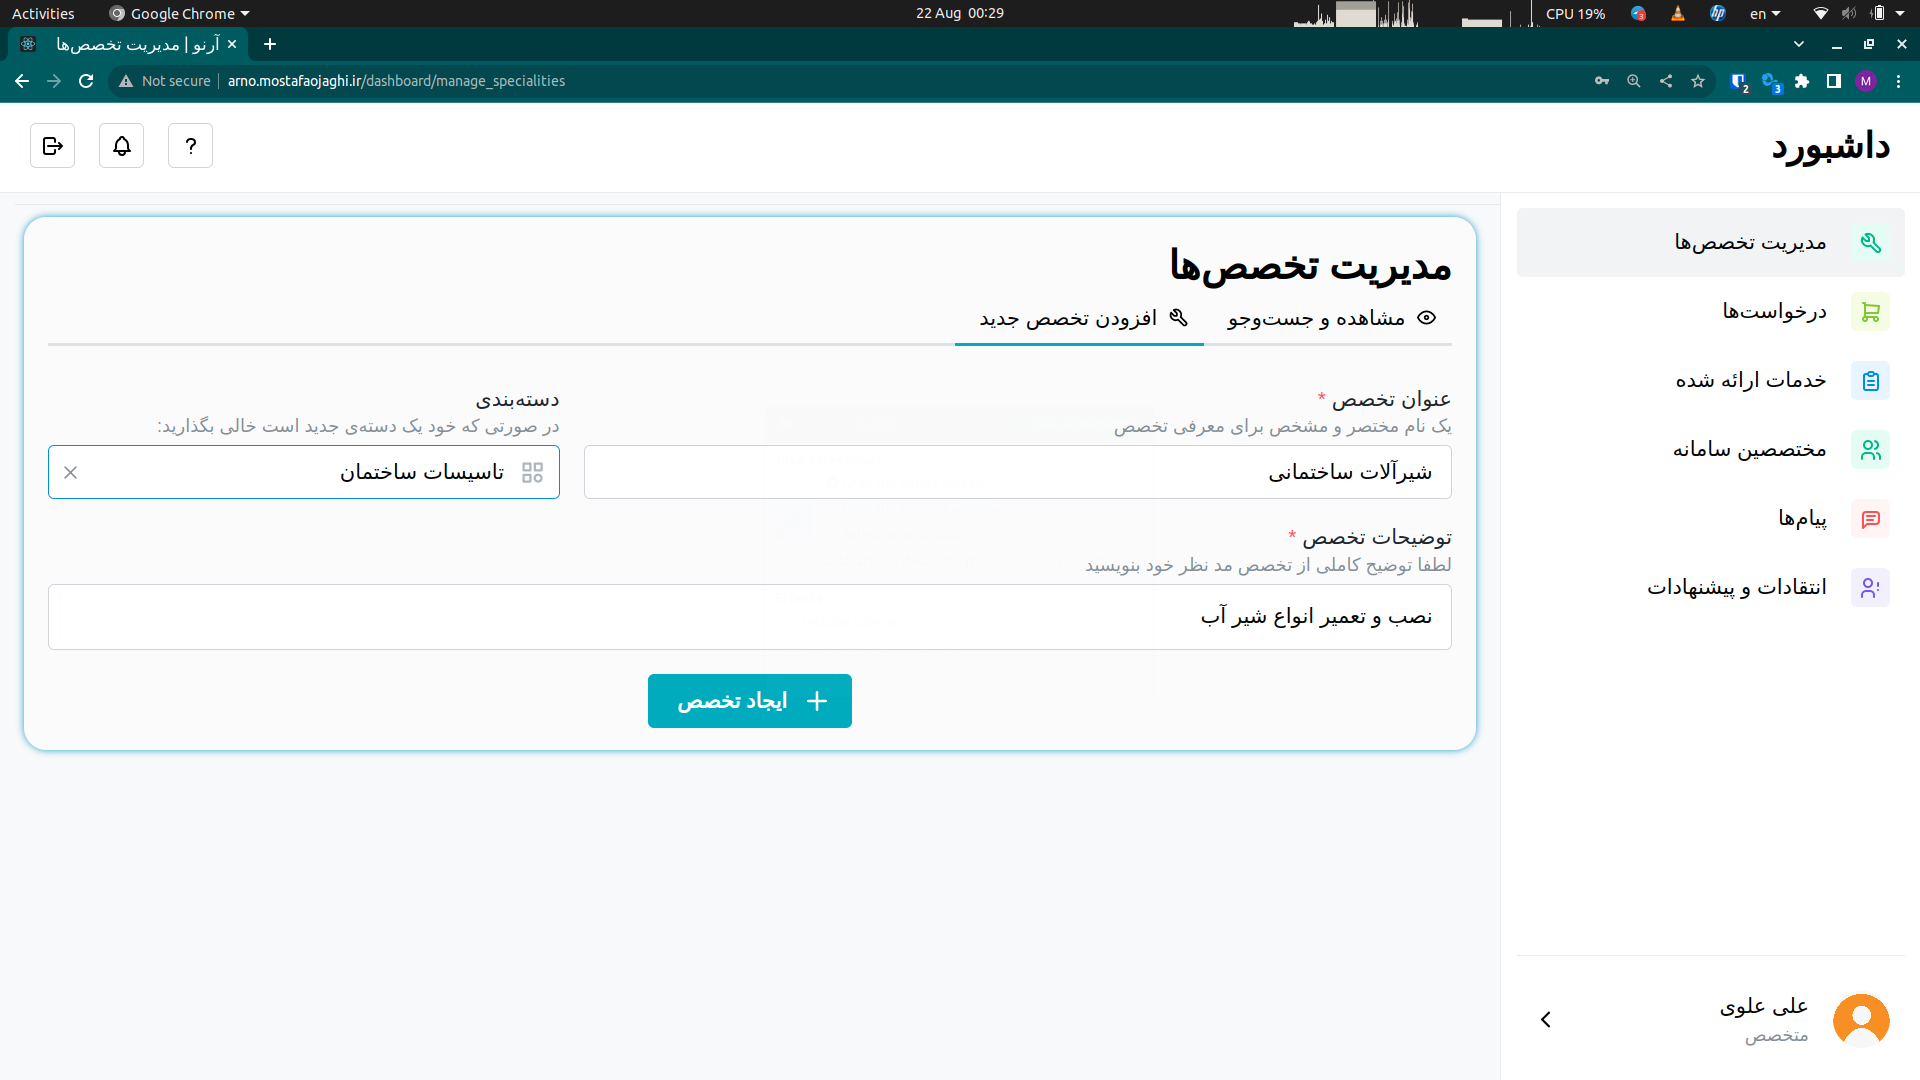
\includegraphics[width=\textwidth]{figs/user-guide/specialist-add-speciality}
	\caption{افزودن تخصص}
	\label{specialist-add-speciality}
\end{figure}

\begin{figure}[h]
	\centering
	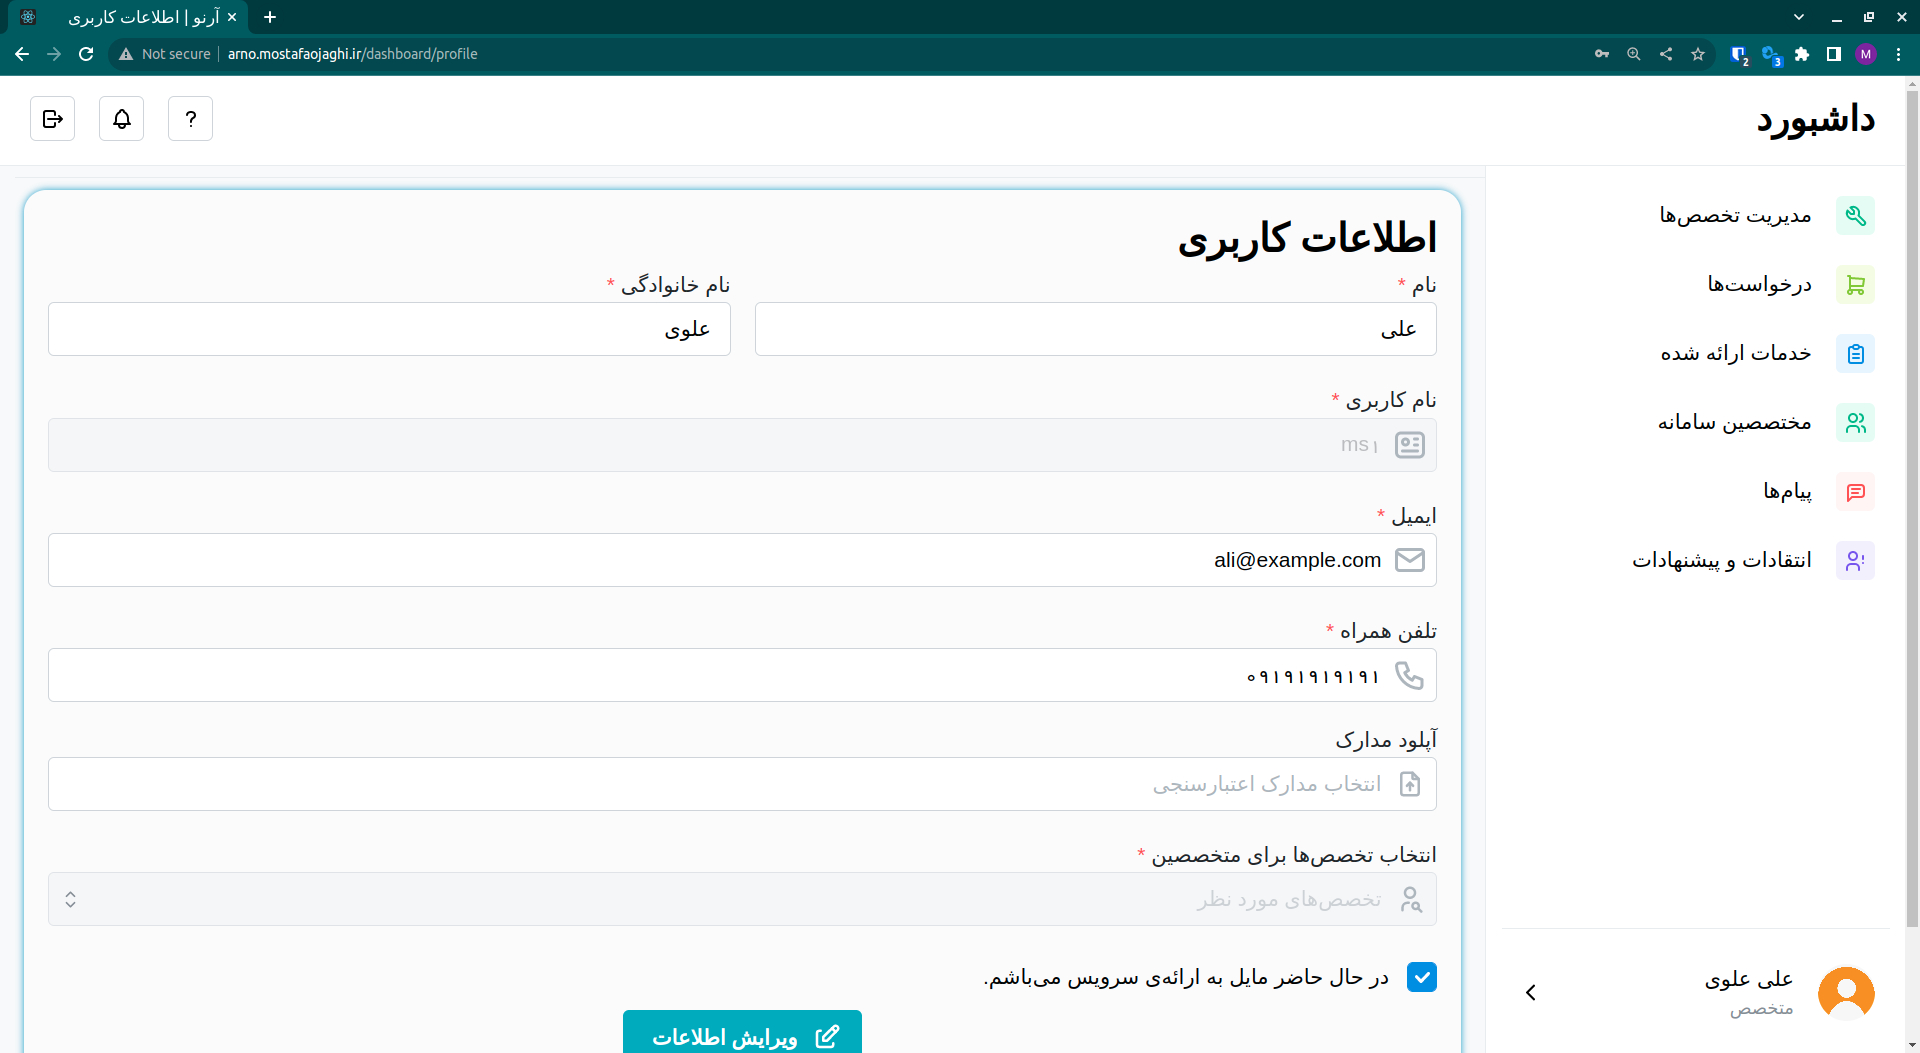
\includegraphics[width=\textwidth]{figs/user-guide/specialist-profile}
	\caption{پروفایل متخصص}
	\label{specialist-profile}
\end{figure}


\FloatBarrier
\section{راهنمای مدیران}

مدیران آرنو می‌توانند مدیران شرکت یا مدیران فنی باشند.
این مدیران باید توسط سایر مدیران ثبت‌نام شوند. 
در این بخش ابتدا به قابلیت‌های مشترک مدیران شرکت و مدیران فنی می‌پردازیم و سپس به موارد اختصاصی هر یک خواهیم پرداخت.

در شکل \ref{tm-dashboard} صفحه‌ی اصلی مدیر فنی و در شکل \ref{cm-dashboard} صفحه‌ی اصلی مدیر شرکت قابل مشاهده است.

\begin{figure}[h]
	\centering
	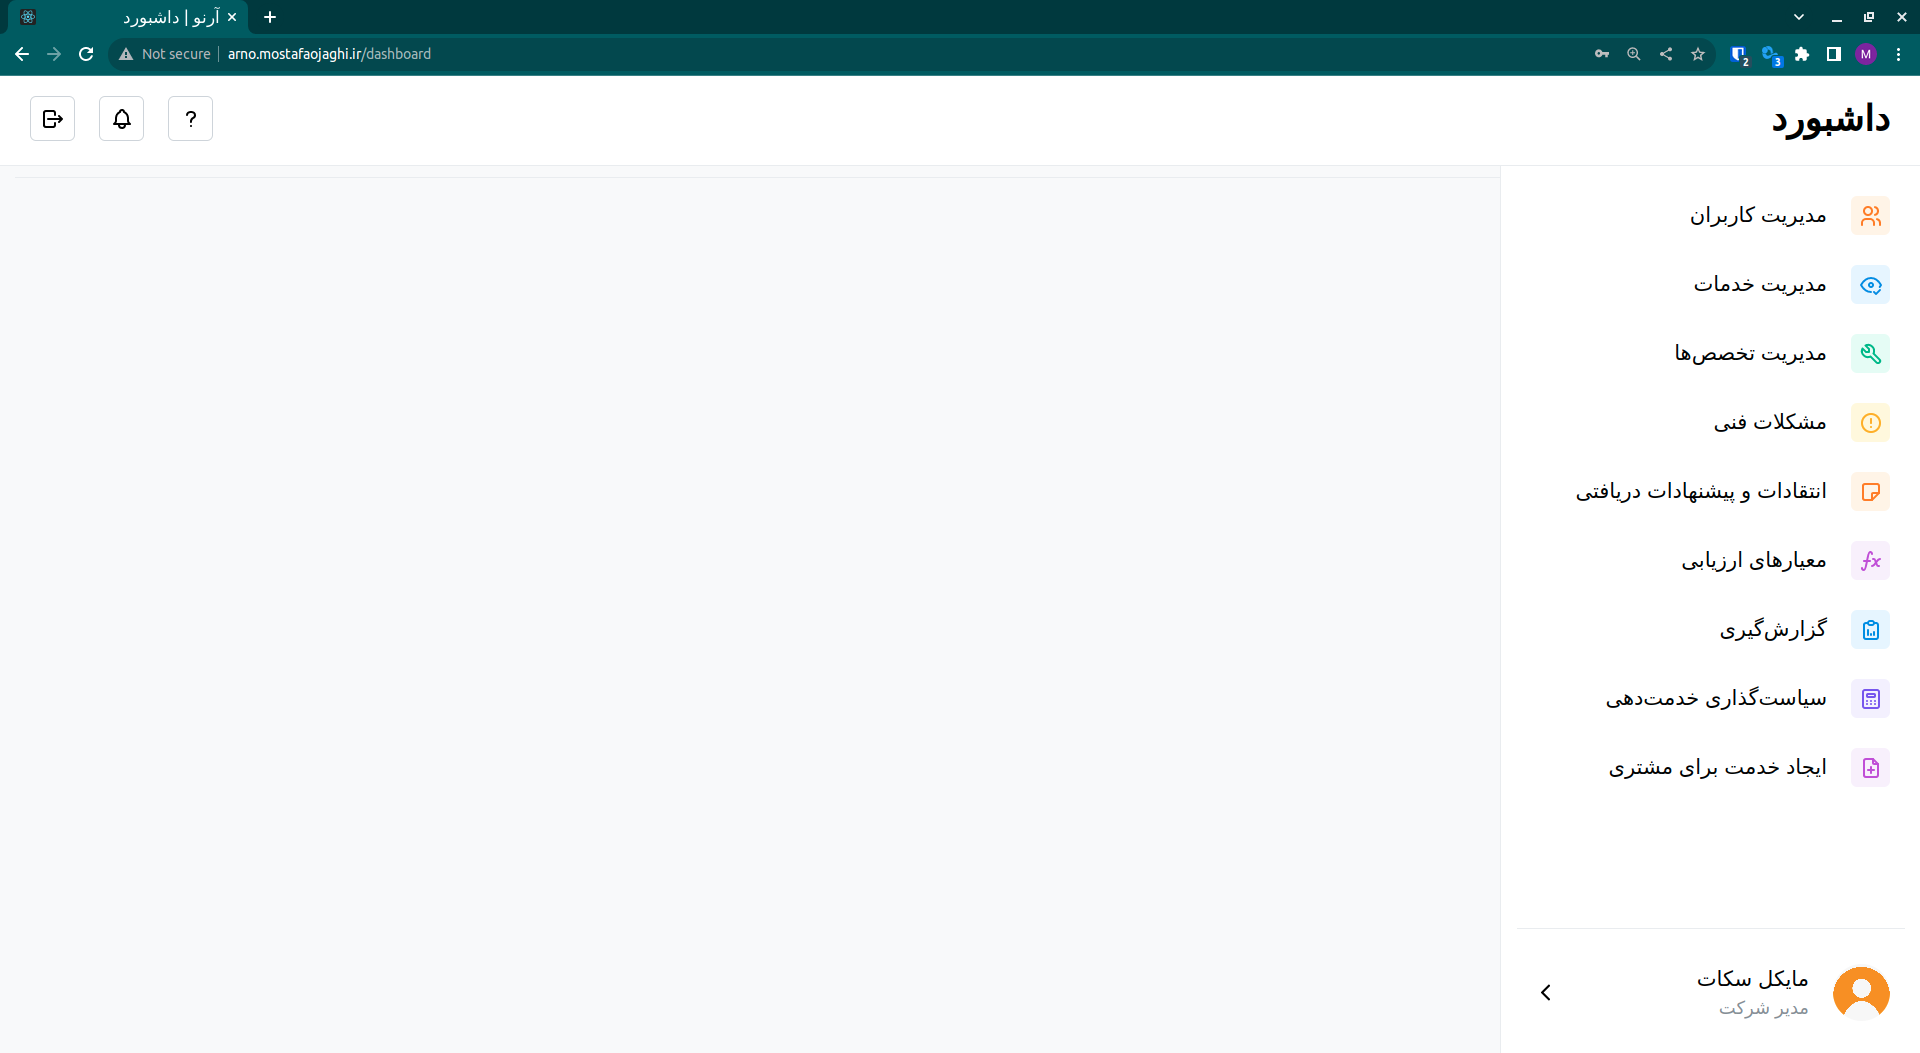
\includegraphics[width=\textwidth]{figs/user-guide/cm-dashboard}
	\caption{صفحه اصلی مدیر شرکت}
	\label{cm-dashboard}
\end{figure}

\begin{figure}[h]
	\centering
	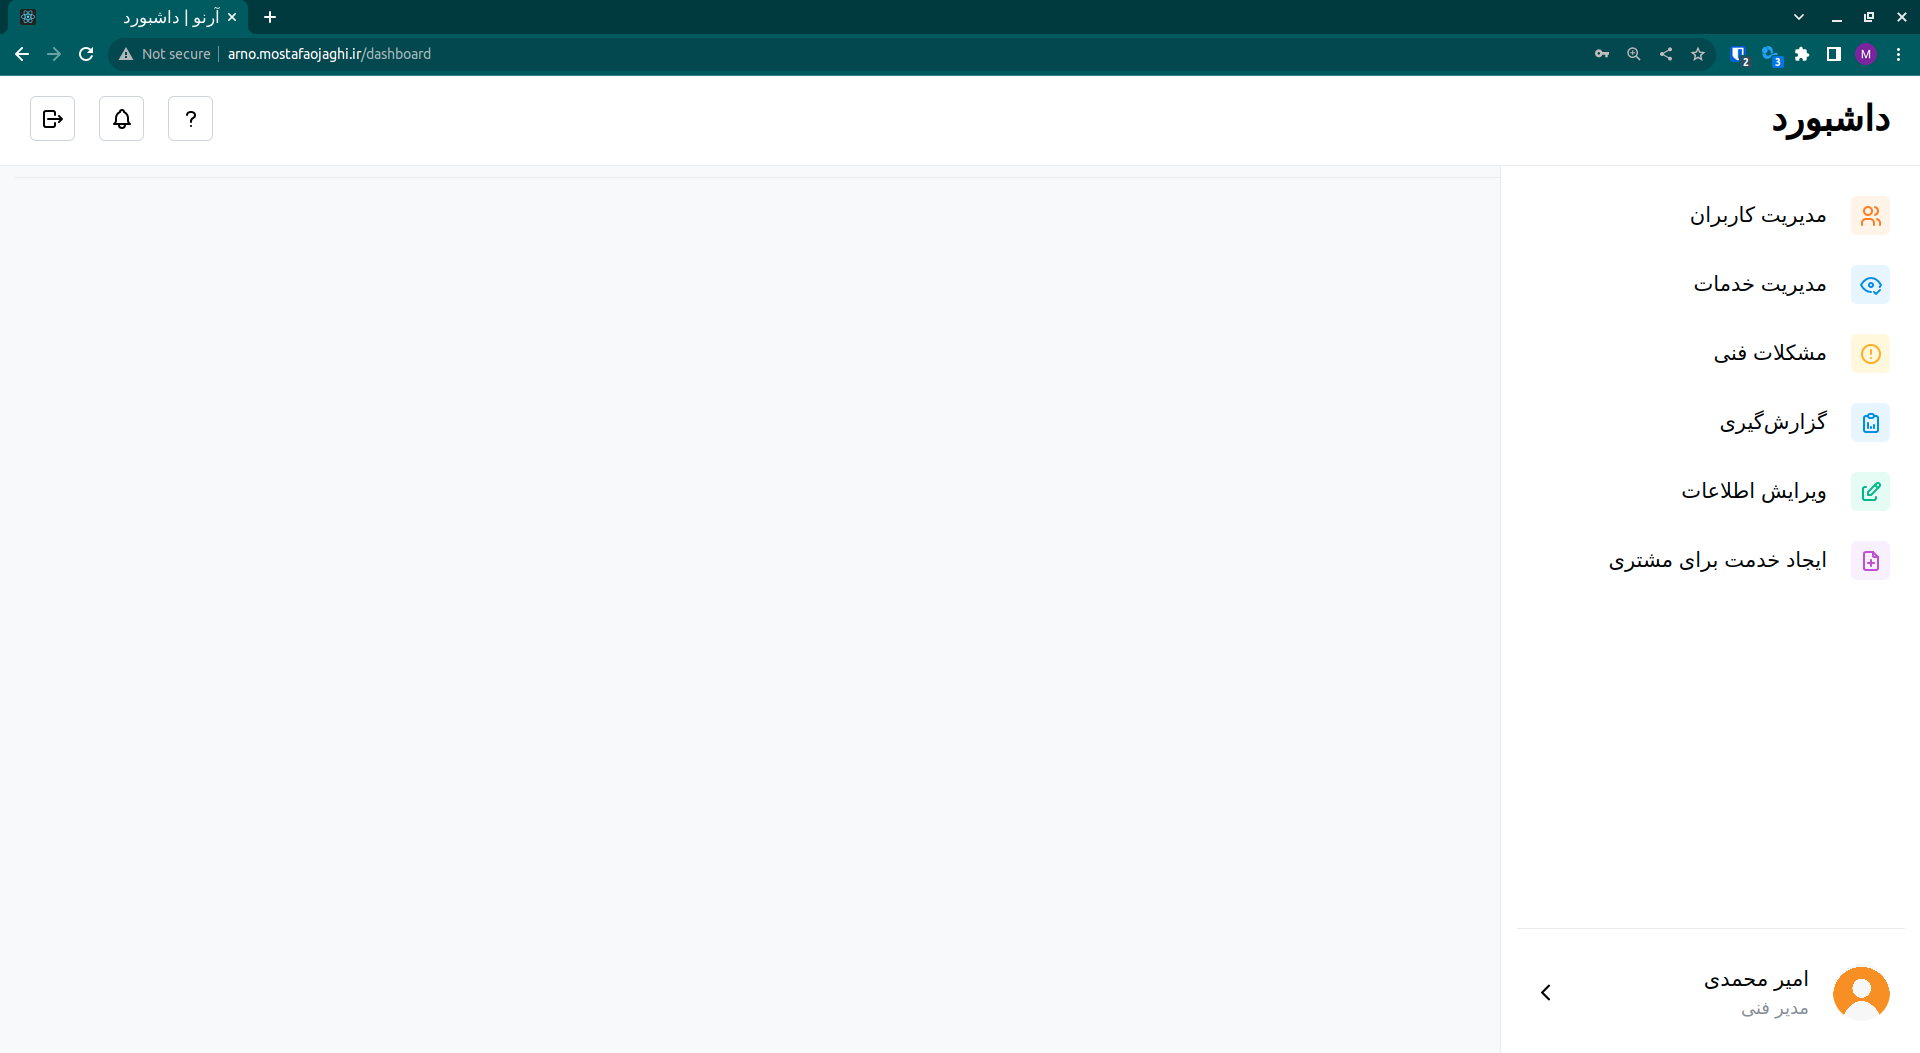
\includegraphics[width=\textwidth]{figs/user-guide/tm-dashboard}
	\caption{صفحه اصلی مدیر فنی}
	\label{tm-dashboard}
\end{figure}

\FloatBarrier

در منوی مدیریت کاربران می‌توان بین کاربران بر اساس موارد مختلف جست و جو انجام داد و جزییات این کاربران را مشاهده کرد.(شکل \ref{manage-users})
برای تایید متخصصان جدید نیز در این منو سربرگ مجزایی وجود دارد که امکان بررسی و تایید متخصصان را در اختیار مدیر قرار می‌دهد.
همچنین در سربرگ آخر این منو می‌توان مدیران جدید را به سامانه اضافه کرد. (شکل \ref{add-manager})

\begin{figure}[h]
	\centering
	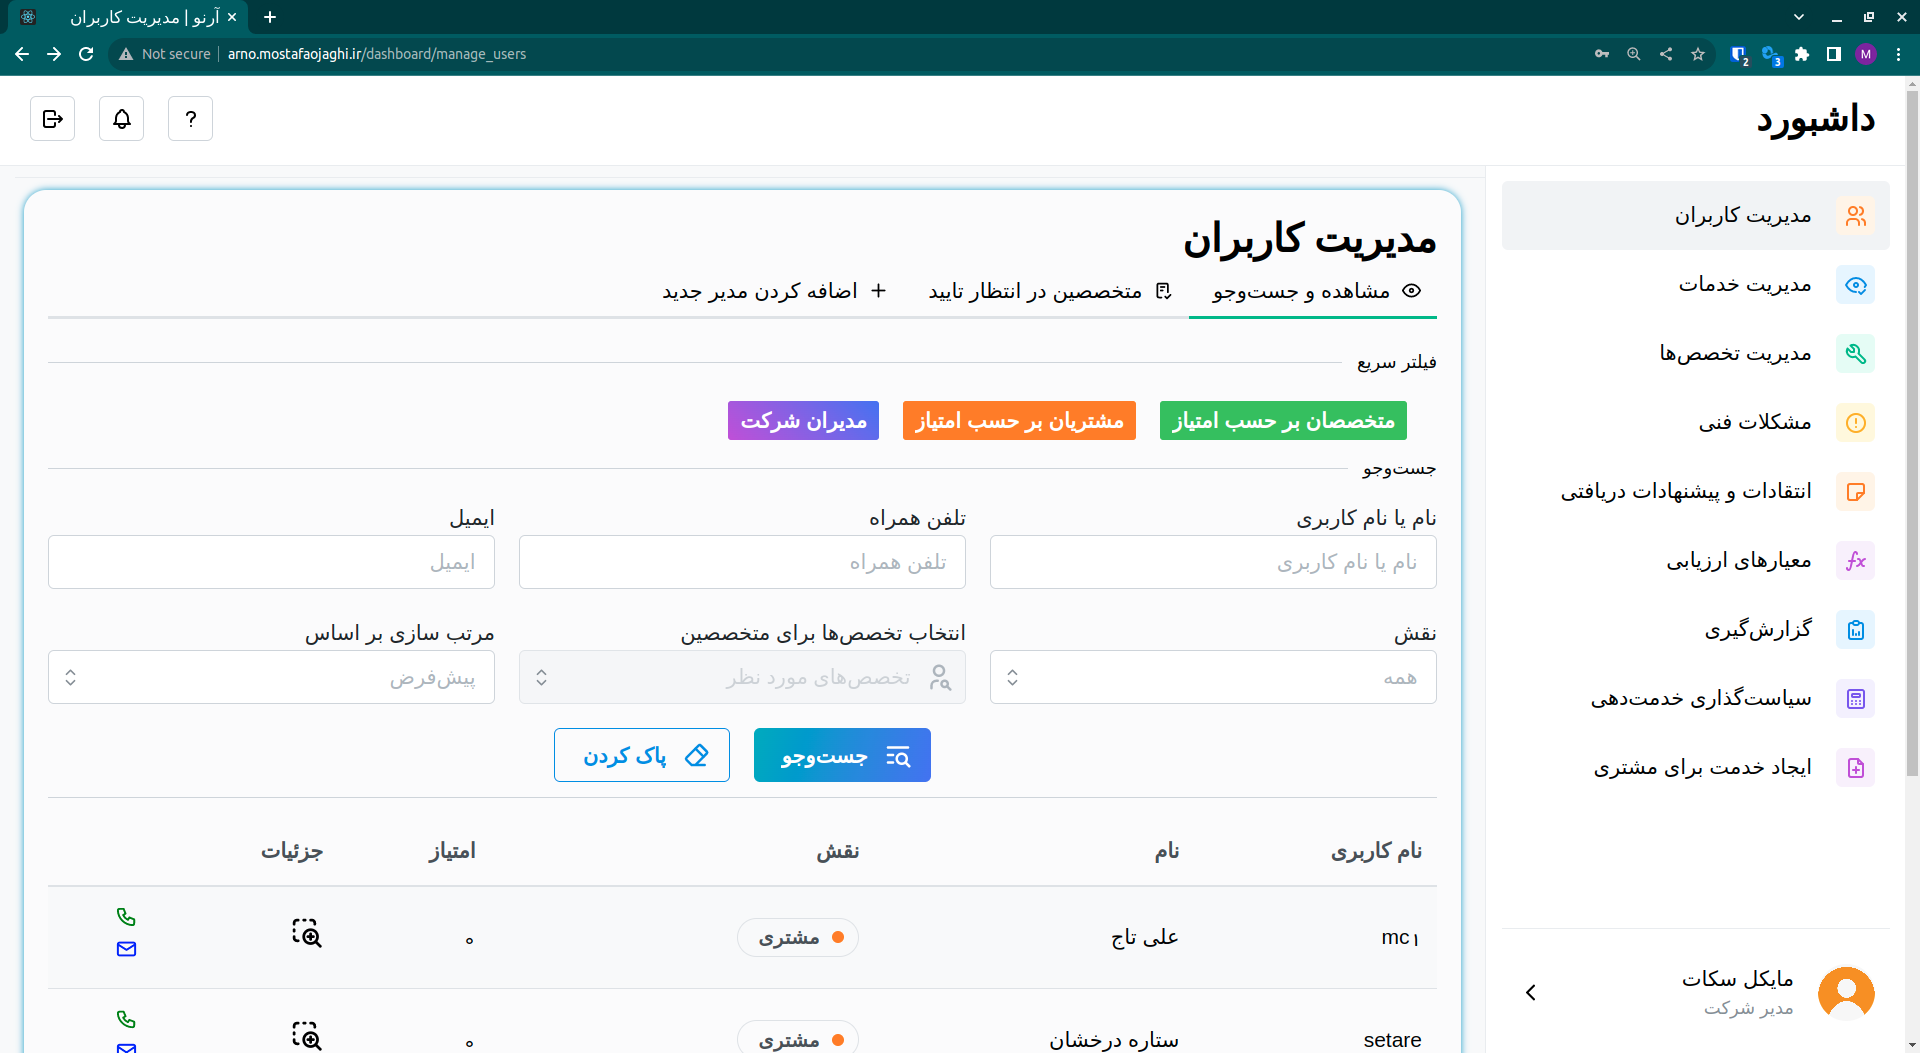
\includegraphics[width=\textwidth]{figs/user-guide/cm-manage-users}
	\caption{صفحه مدیریت کاربران}
	\label{manage-users}
\end{figure}

\begin{figure}[h]
	\centering
	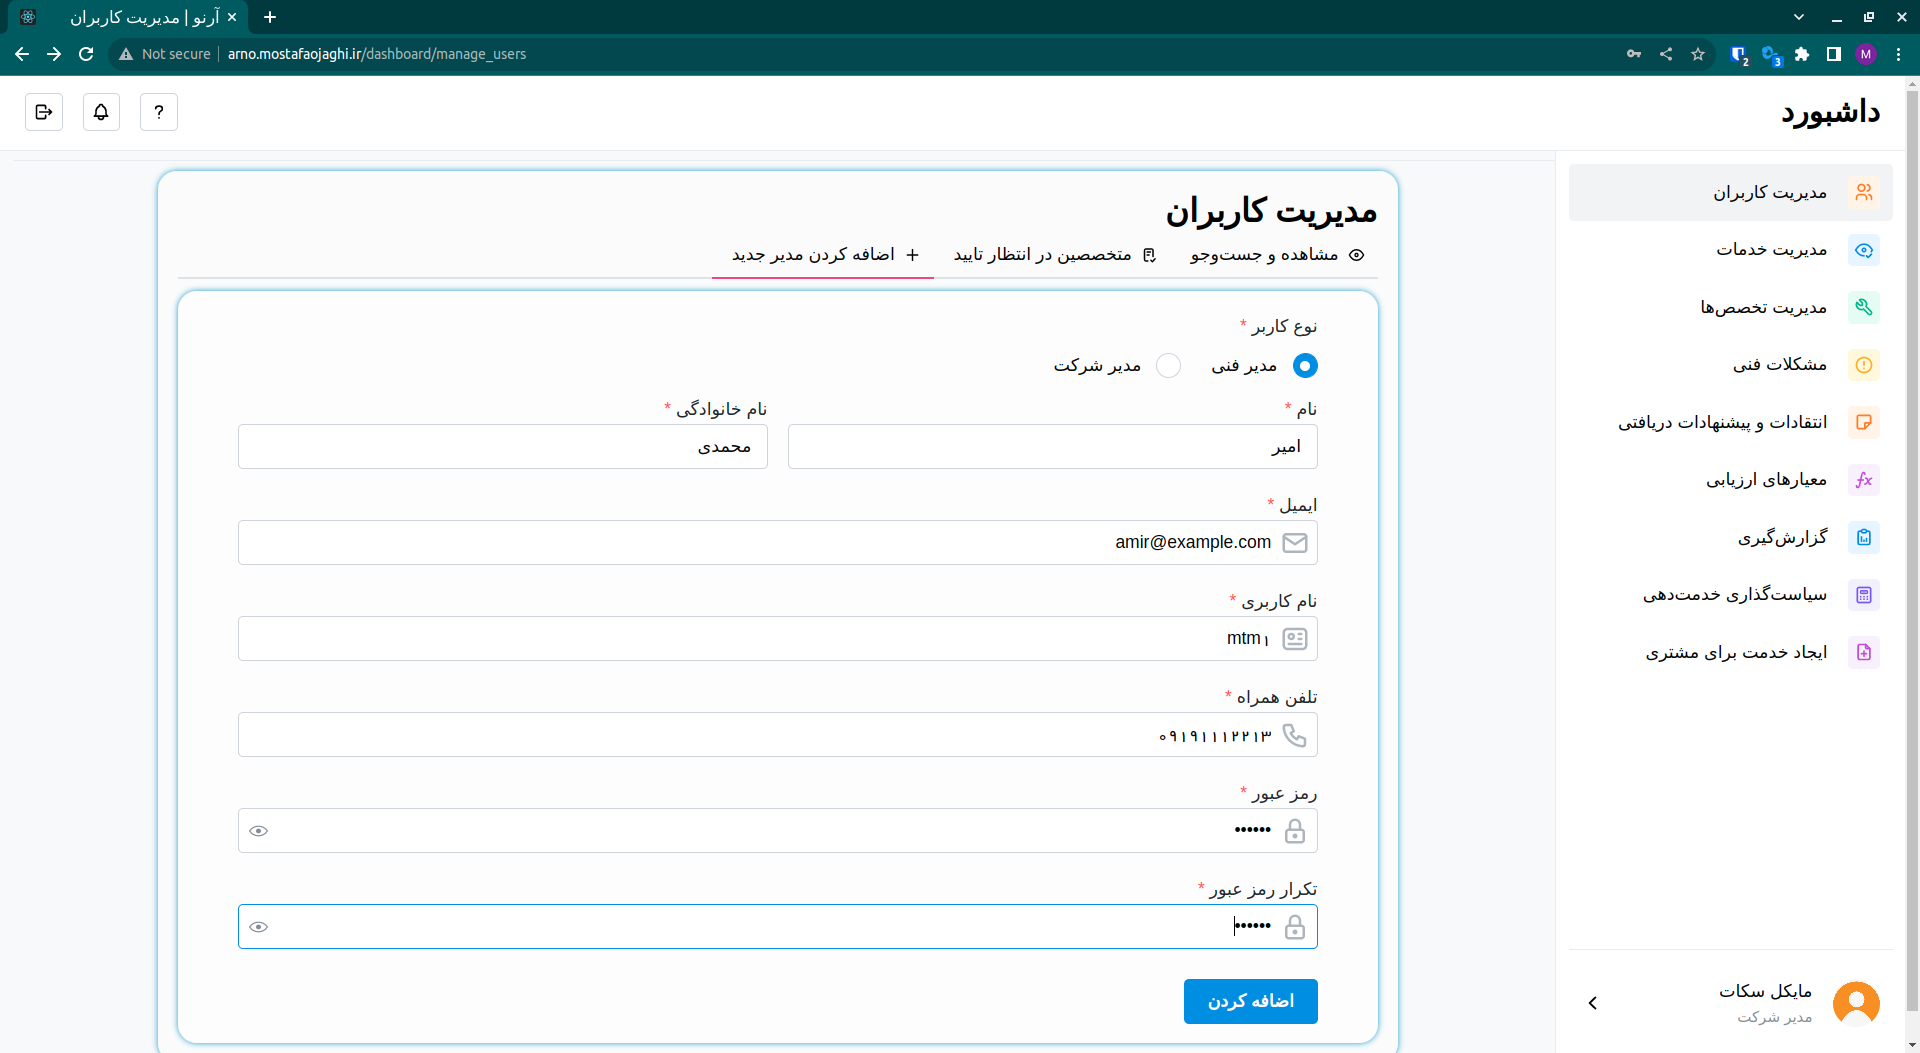
\includegraphics[width=\textwidth]{figs/user-guide/cm-add-manager}
	\caption{صفحه افزودن مدیر جدید}
	\label{add-manager}
\end{figure}

\FloatBarrier

در منوی مدیریت خدمات (شکل \ref{manage-requests}) می‌توان خدمات درخواست شده را مشاهده کرده و روی آن‌ها جست و جو انجام داد.
همچنین در صورت نیاز امکان لغو خدمت در این منو وجود دارد.
در این قسمت سربرگ جداگانه‌ای نیز برای مشاهده‌ی خدماتی که در یک بازه‌ی زمانی خاص درخواست شده اند ولی متخصصی آن‌ها را ارائه نکرده است تعبیه شده‌است.

\begin{figure}[h]
	\centering
	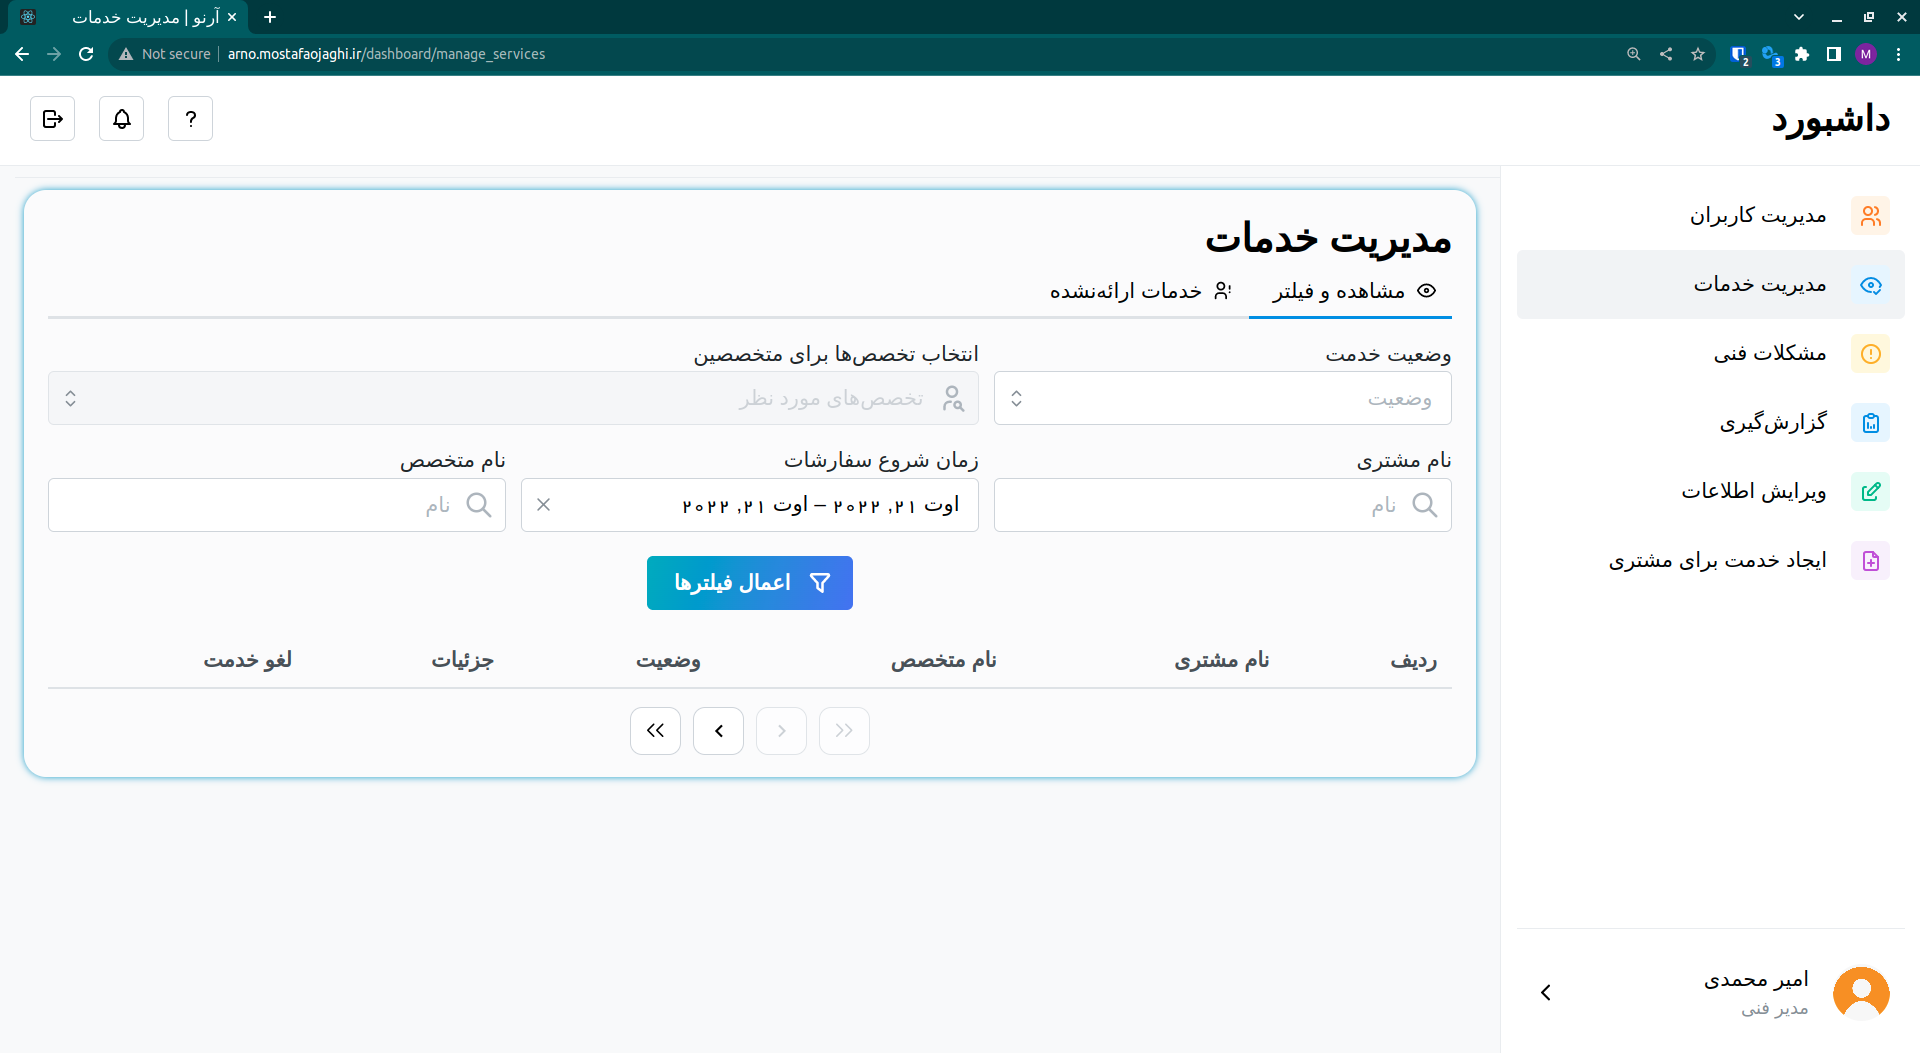
\includegraphics[width=\textwidth]{figs/user-guide/tm-manage-requests}
	\caption{صفحه افزودن مدیر جدید}
	\label{manage-requests}
\end{figure}

\FloatBarrier

منوی مشترک بعدی، منوی گزارش‌گیری (شکل \ref{system-report}) است که به کمک آن می‌توان لاگ‌های سیستم را فیلتر و مشاهده کرد.
این منو برای بررسی و رفع خطاها و مشکلات سیستم کاربرد دارد.

آخرین منوی مشترک نیز منوی ایجاد خدمت برای مشتری (شکل \ref{create-request-for-user}) است.
در این منو مدیر شرکت می‌تواند در موارد مورد نیاز خدمتی را برای یک مشتری خاص درخواست کند.

\begin{figure}[h]
	\centering
	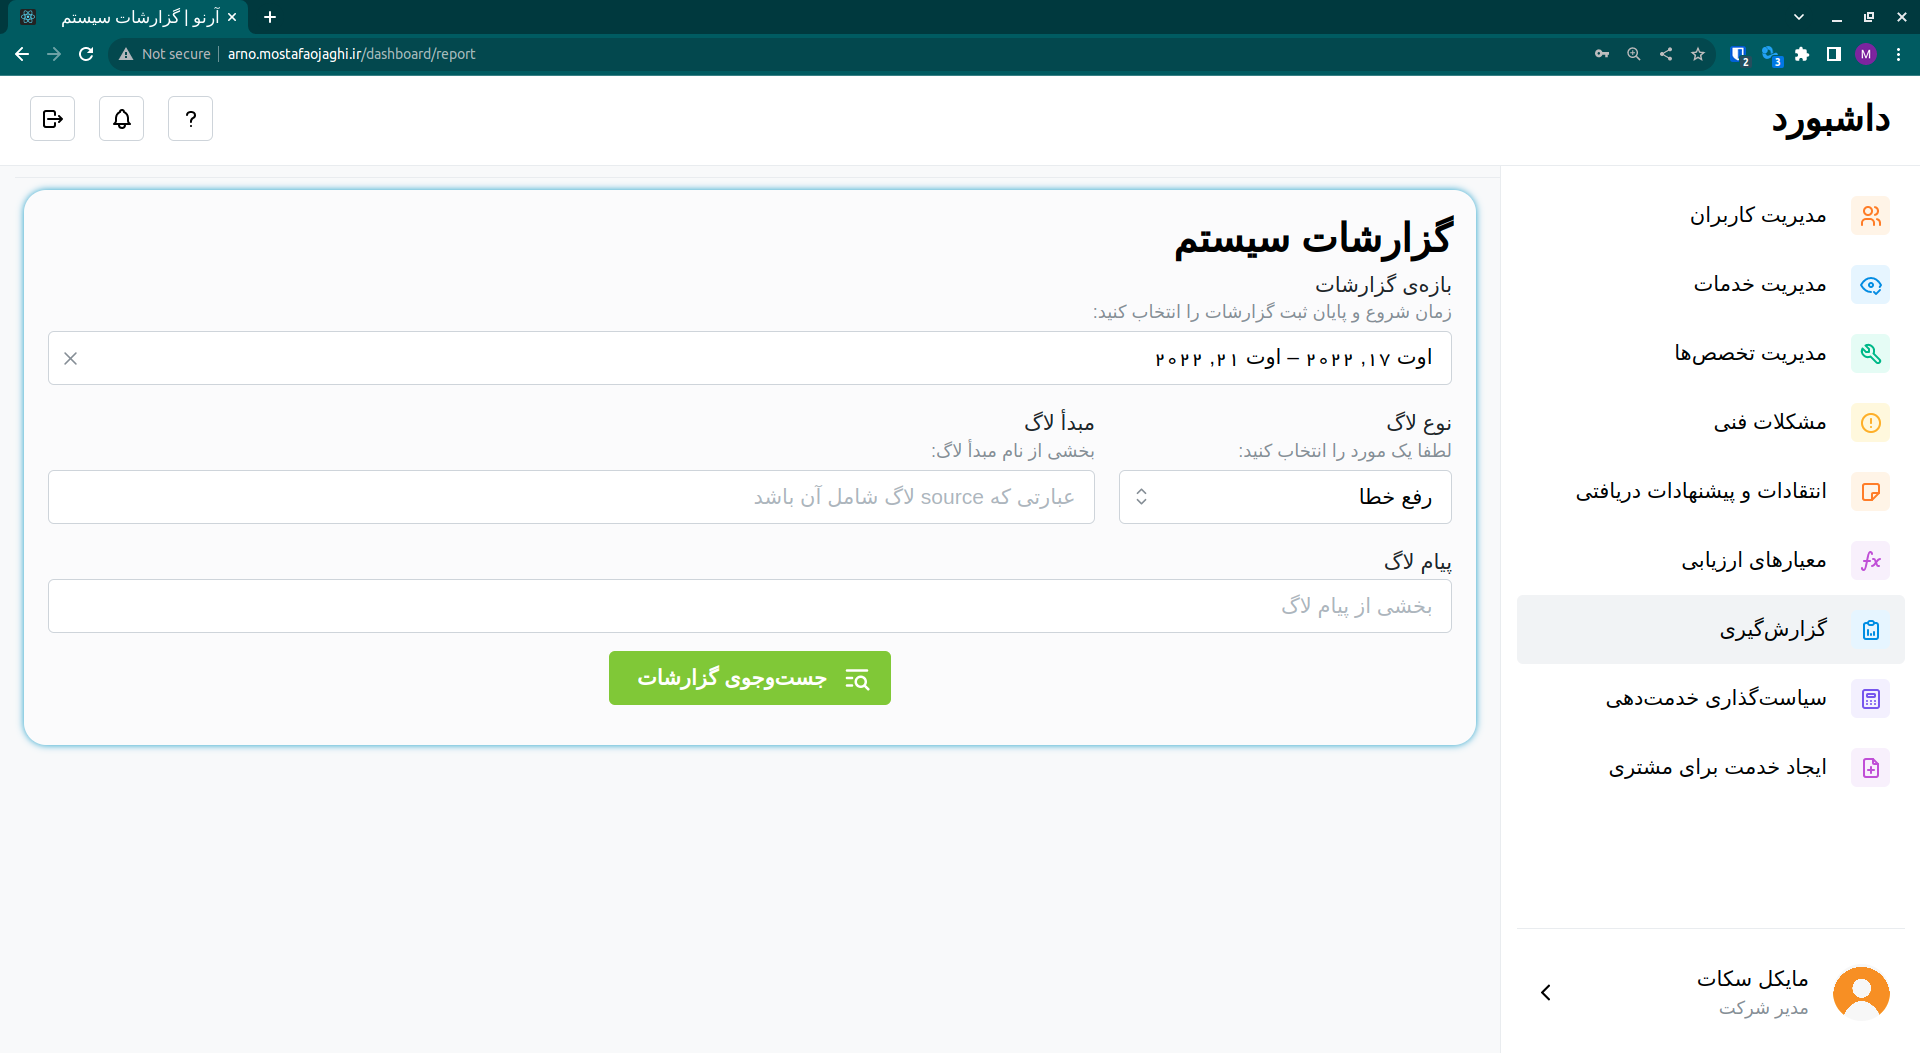
\includegraphics[width=\textwidth]{figs/user-guide/cm-report}
	\caption{صفحه گزارش‌گیری}
	\label{system-report}
\end{figure}

\begin{figure}[h]
	\centering
	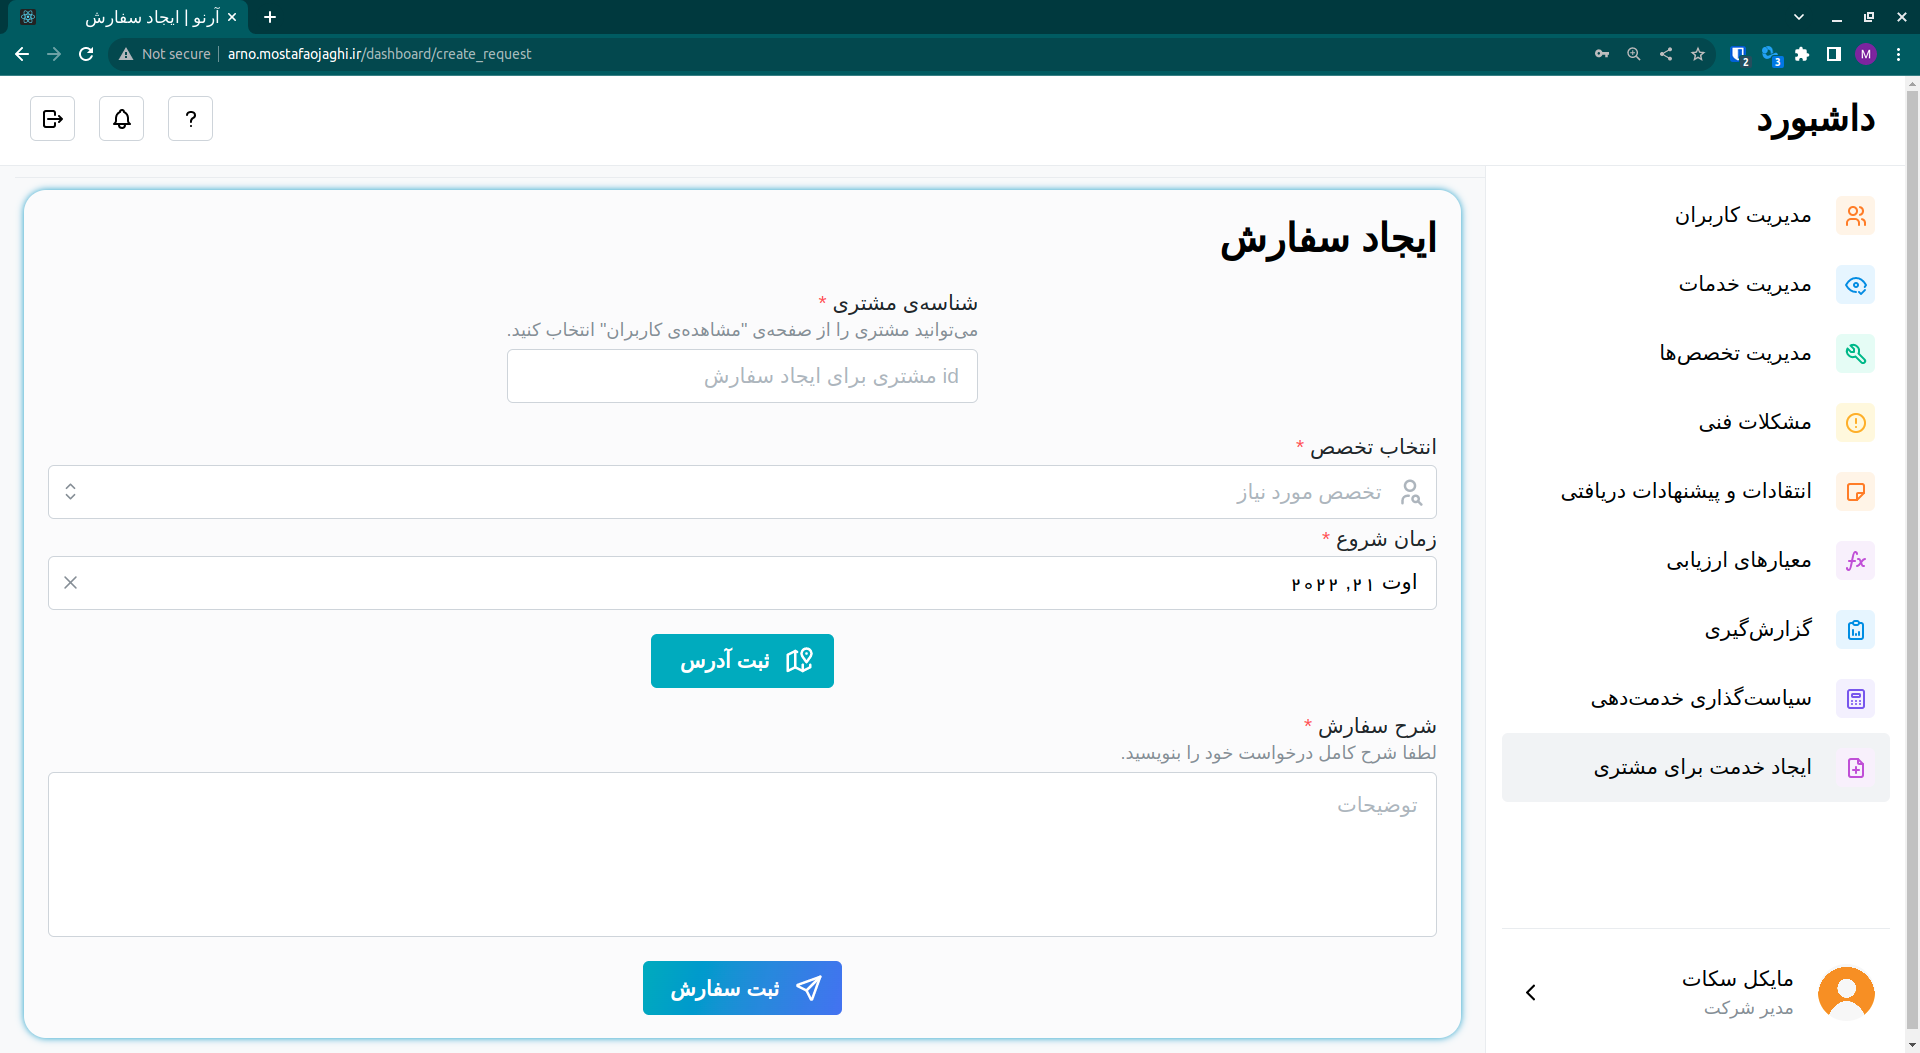
\includegraphics[width=\textwidth]{figs/user-guide/cm-create-request}
	\caption{صفحه ایجاد خدمت برای مشتری}
	\label{create-request-for-user}
\end{figure}

\FloatBarrier

مدیران فنی علاوه بر موارد فوق امکان مشاهده و پاسخ به گزارش مشکلات فنی و همچنین ویرایش اطلاعات را دارند.
همین‌طور برای مدیران شرکت نیز چهار منوی اختصاصی وجود دارد که به ترتیب توضیح داده می‌شوند.

خدمات آرنو در تخصص‌هایی مشخص انجام می‌شود که در دسته‌های کلی‌تری برای کاربری بهتر قرار می‌گیرند.
مدیر شرکت با استفاده از منوی مدیریت تخصص‌ها (شکل \ref{cm-manage-specialities})  می‌تواند این دسته‌ها و تخصص‌ها را مشاهده کرده، دسته‌ها و تخصص‌های جدیدی به آن‌ها بیافزاید.
برای افزودن یک تخصص ابتدا باید دسته‌ای برای آن ایجاد شود. برای این کار در منوی افزودن تخصص جدید (شکل \ref{cm-add-category}) باید یک تخصص بدون مشخص کردن دسته افزوده شود.
سپس می‌توان دسته‌ی افزوده شده را برای تخصص‌های جدید انتخاب کرد.(شکل \ref{cm-add-speciality})
در آخرین سربرگ این منو هم می‌توان تخصص‌ها را در یک بازه‌ی زمانی مشخص برحسب تعداد درخواست صورت‌گرفته برای آن‌ها مرتب کرد.

\begin{figure}[h]
	\centering
	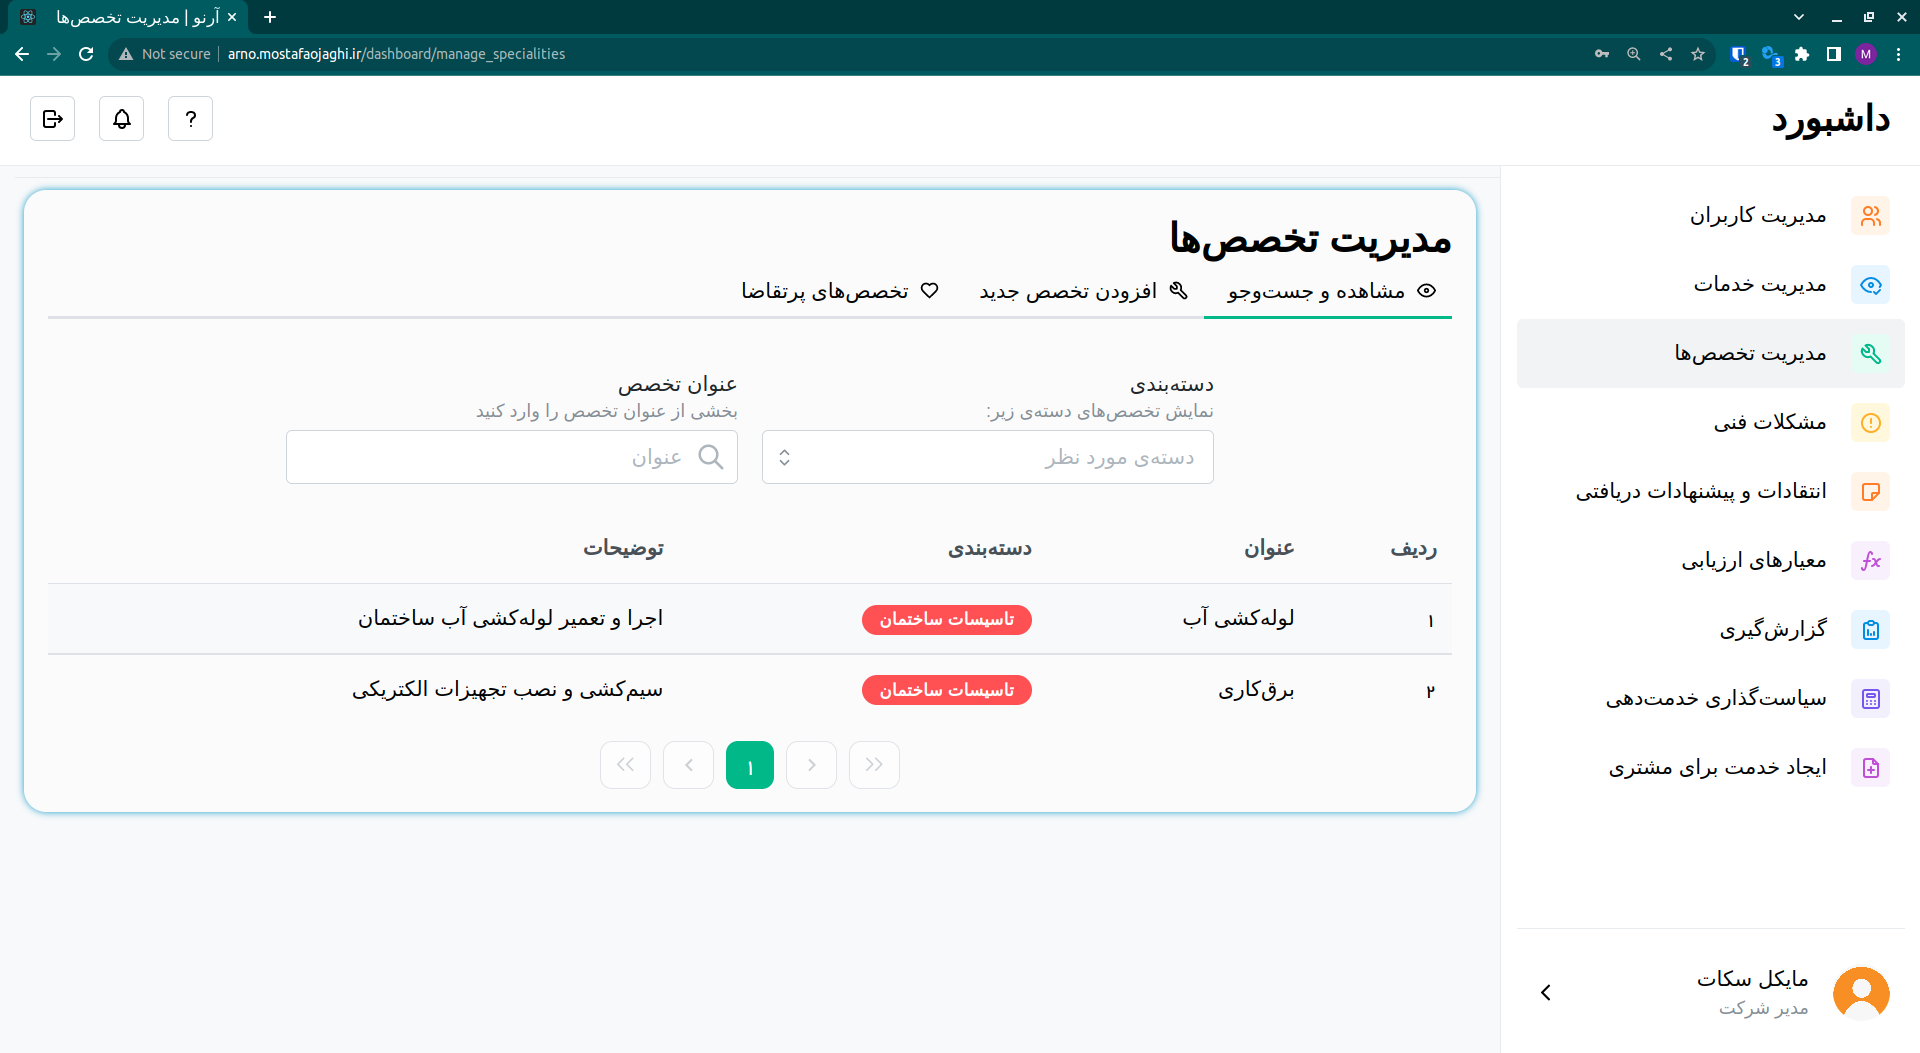
\includegraphics[width=\textwidth]{figs/user-guide/cm-manage-specialities}
	\caption{صفحه مدیریت تخصص‌ها}
	\label{cm-manage-specialities}
\end{figure}

\begin{figure}[h]
	\centering
	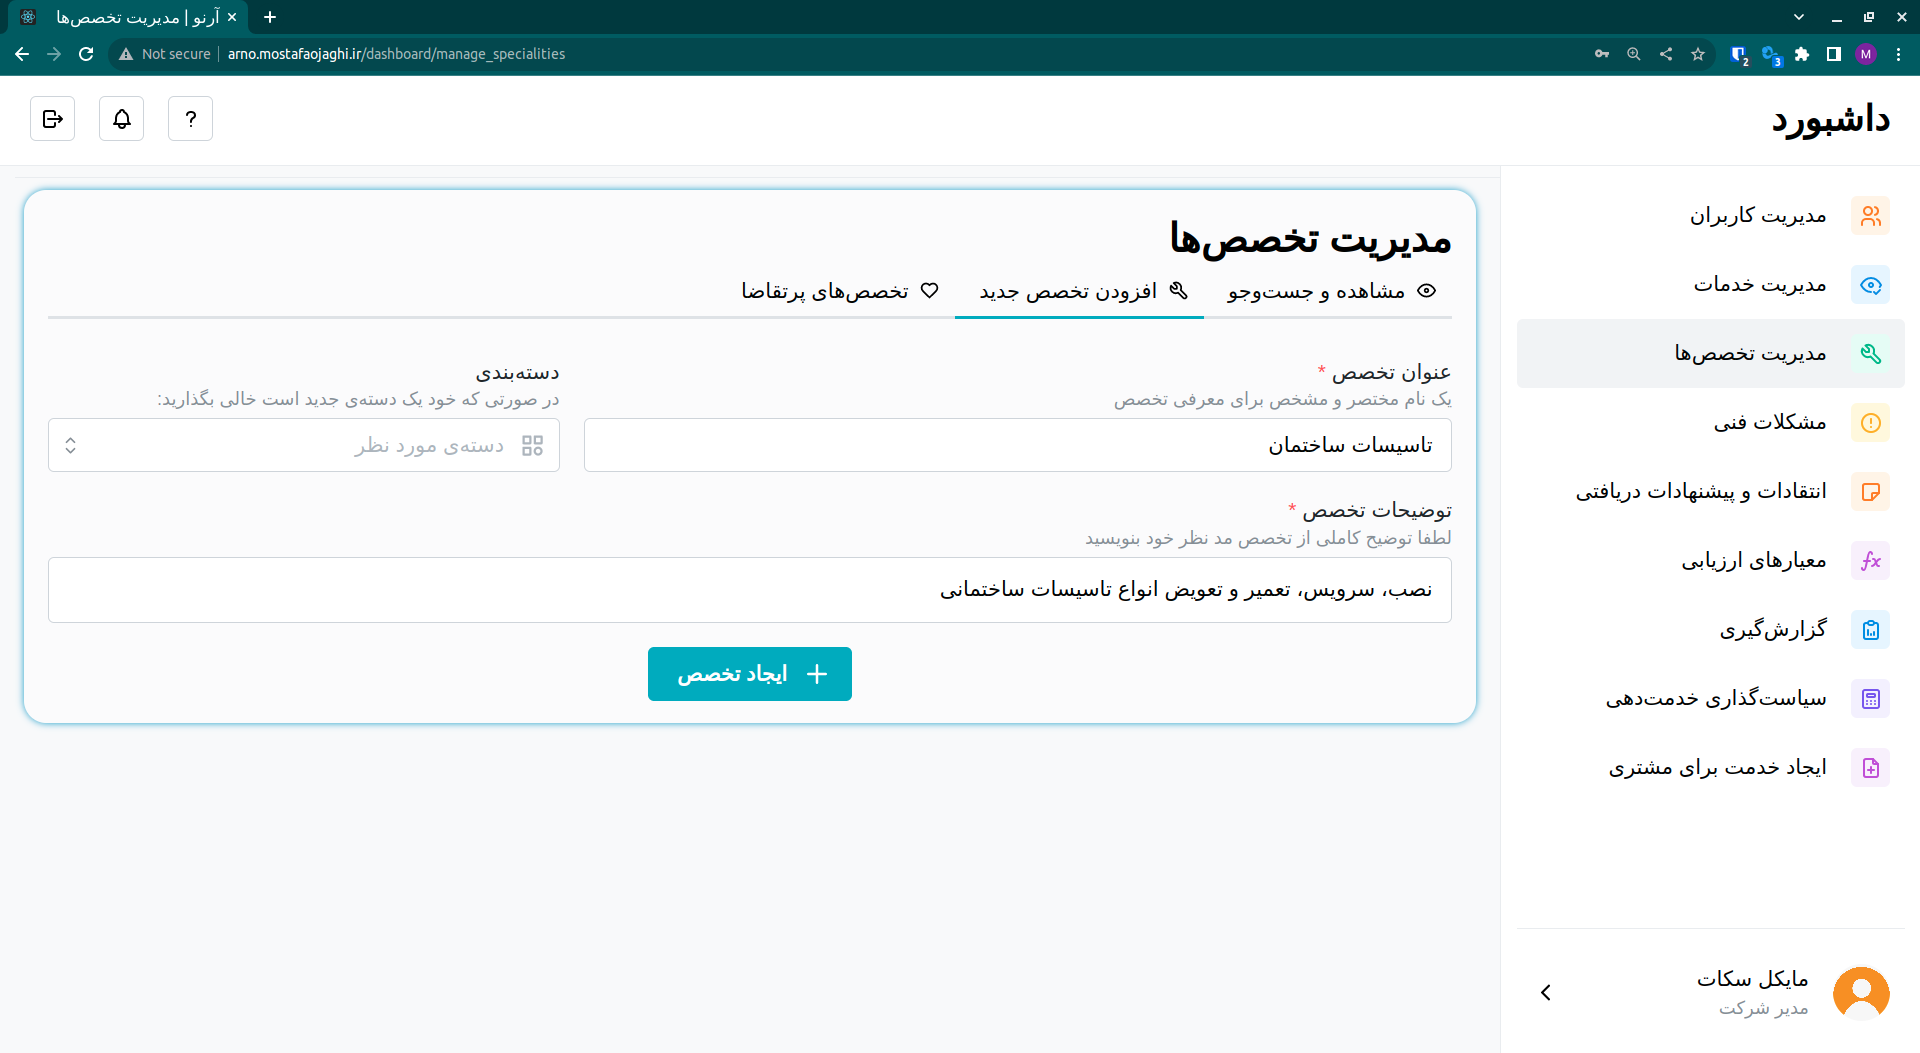
\includegraphics[width=\textwidth]{figs/user-guide/cm-add-category}
	\caption{افزودن دسته‌ تخصص}
	\label{cm-add-category}
\end{figure}

\begin{figure}[h]
	\centering
	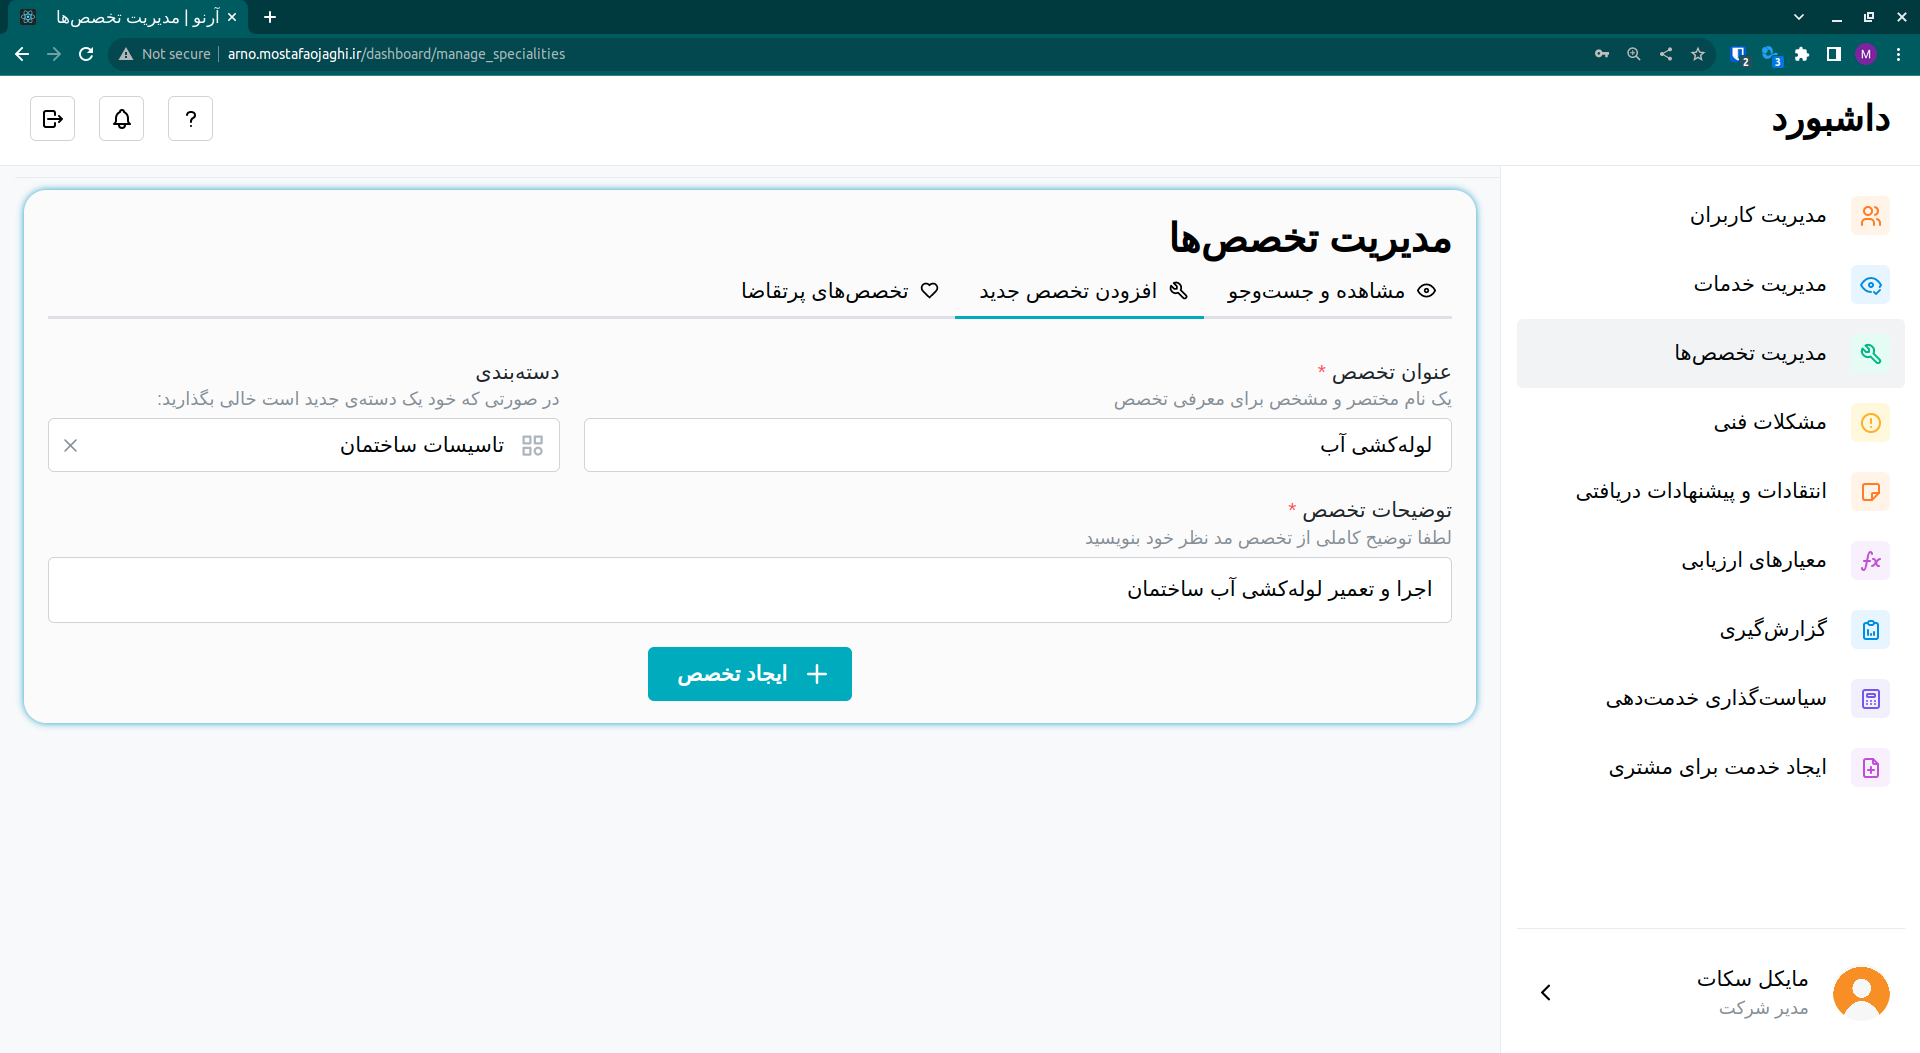
\includegraphics[width=\textwidth]{figs/user-guide/cm-add-speciality}
	\caption{افزودن تخصص}
	\label{cm-add-speciality}
\end{figure}

\FloatBarrier

آرنو امکان ارزیابی متخصصان را به مشتریان و امکان ارزیابی مشتریان را به متخصصان می‌دهد.
این ارزیابی به صورت کمی (نیم ستاره تا پنج ستاره) انجام می‌شود و بر روی تعداد درخواست‌های همزمانی که یک متخصص می‌تواند بپذیرد تاثیر گذار است.
برای مدیریت این عملکرد دو منوی معیارهای ارزیابی و سیاست‌گذاری خدمت‌دهی تعبیه شده اند.
در منوی معیارهای ارزیابی می‌توان معیارهای موجود را ویرایش یا حذف کرد.(شکل \ref{cm-evaluation-metrics})
برای افزودن معیارهای جدید هم می‌توان از دکمه‌ی بالای این صفحه استفاده کرد.
با فشردن این دکمه صفحه‌ی شکل \ref{cm-add-evaluation-metric} باز می‌شود و از طریق آن می‌توان معیار دلخواه را اضافه کرد.
پس از پایان انجام هر خدمت کاربران یکدیگر را ارزیابی کرده و میانگین این معیارها به عنوان امتیاز کسب شده از آن خدمت در نظر گرفته می‌شود.
در منوی سیاست‌گذاری خدمت‌دهی می‌توان بر اساس میانگین امتیازهای کسب شده توسط یک متخصص، تعداد درخواست‌هایی که می‌تواند به صورت همزمان قبول کند را مشخص کرد.
این کار با افزودن تعدادی سیاست انجام می‌شود.
هر سیاست شامل یک حداقل امتیاز و تعداد درخواست‌هایی که با داشتن آن امتیاز می‌توان قبول کرد است.
در این منو (شکل \ref{cm-service-policy}) می‌توان این سیاست‌ها را ویرایش، حذف یا اضافه کرد.

\begin{figure}[h]
	\centering
	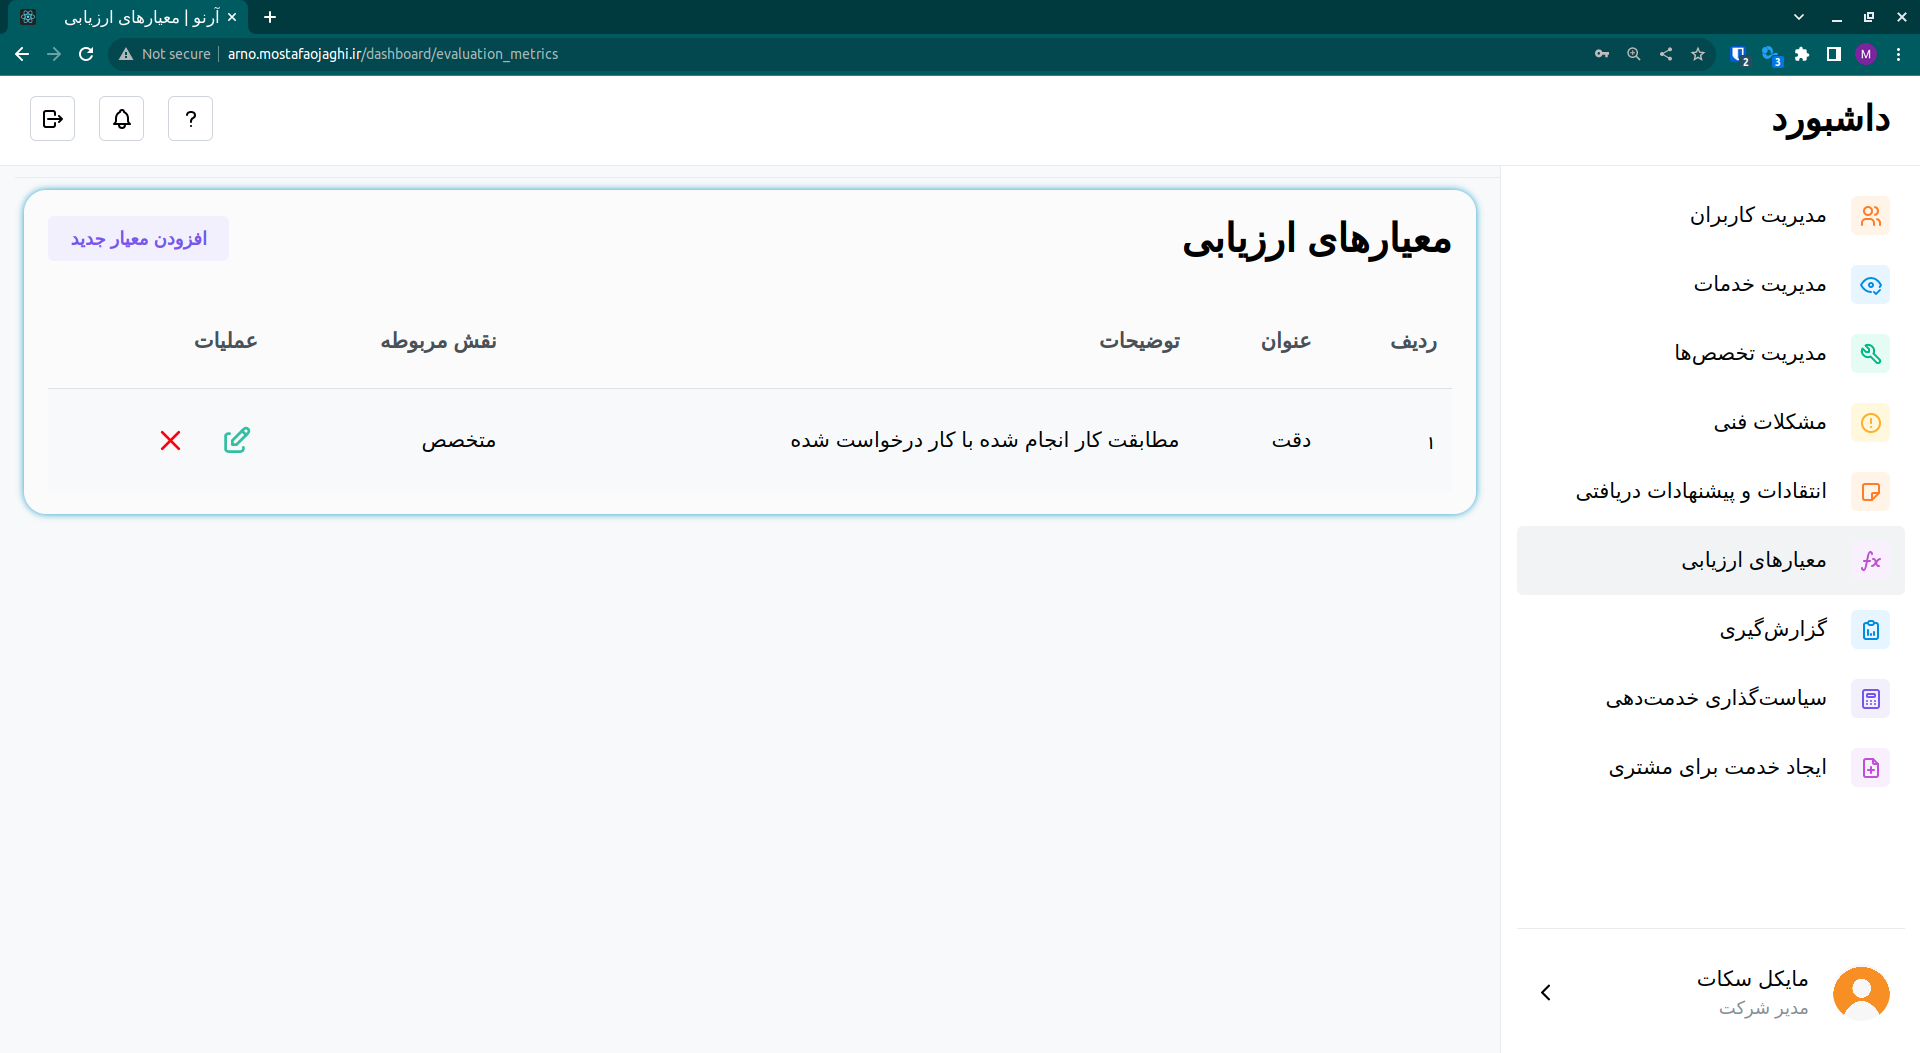
\includegraphics[width=\textwidth]{figs/user-guide/cm-evaluation-metrics}
	\caption{صفحه معیارهای ارزیابی}
	\label{cm-evaluation-metrics}
\end{figure}

\begin{figure}[h]
	\centering
	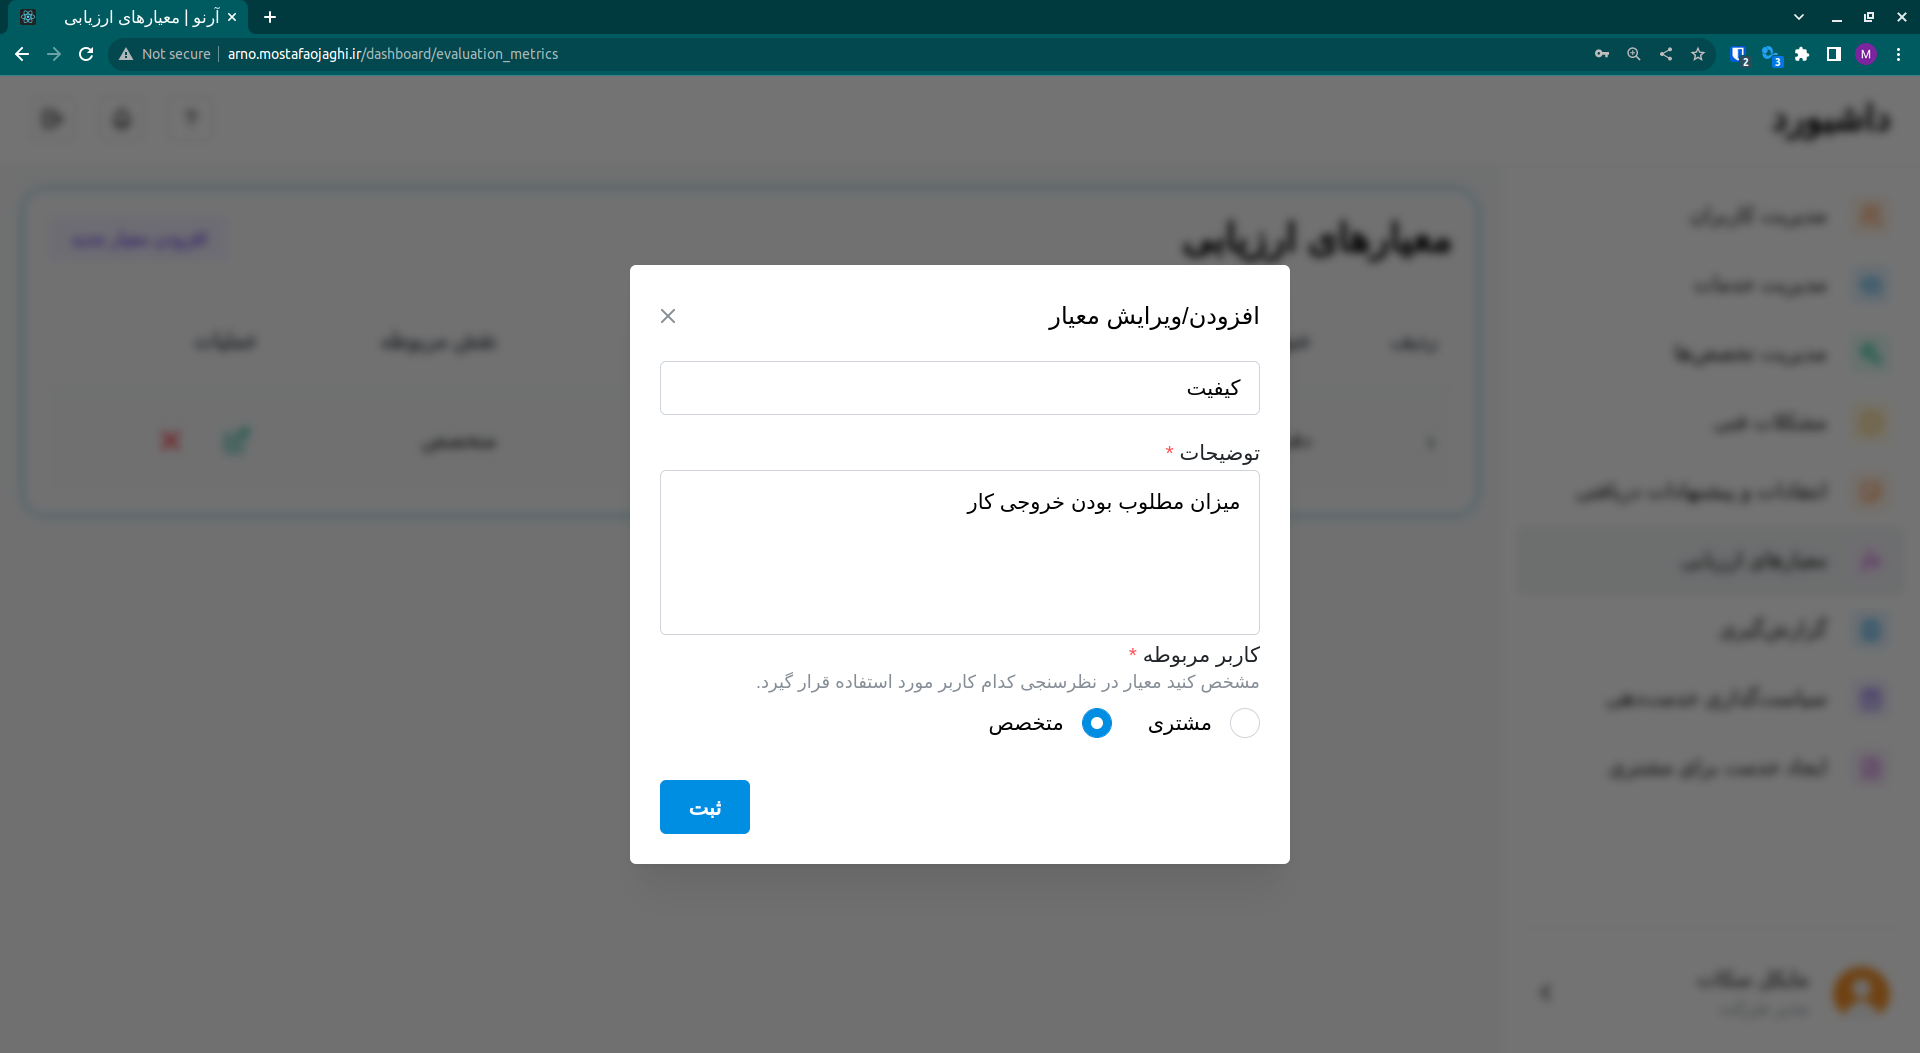
\includegraphics[width=\textwidth]{figs/user-guide/cm-add-evaluation-metric}
	\caption{افزودن میعار ارزیابی}
	\label{cm-add-evaluation-metric}
\end{figure}

\begin{figure}[h]
	\centering
	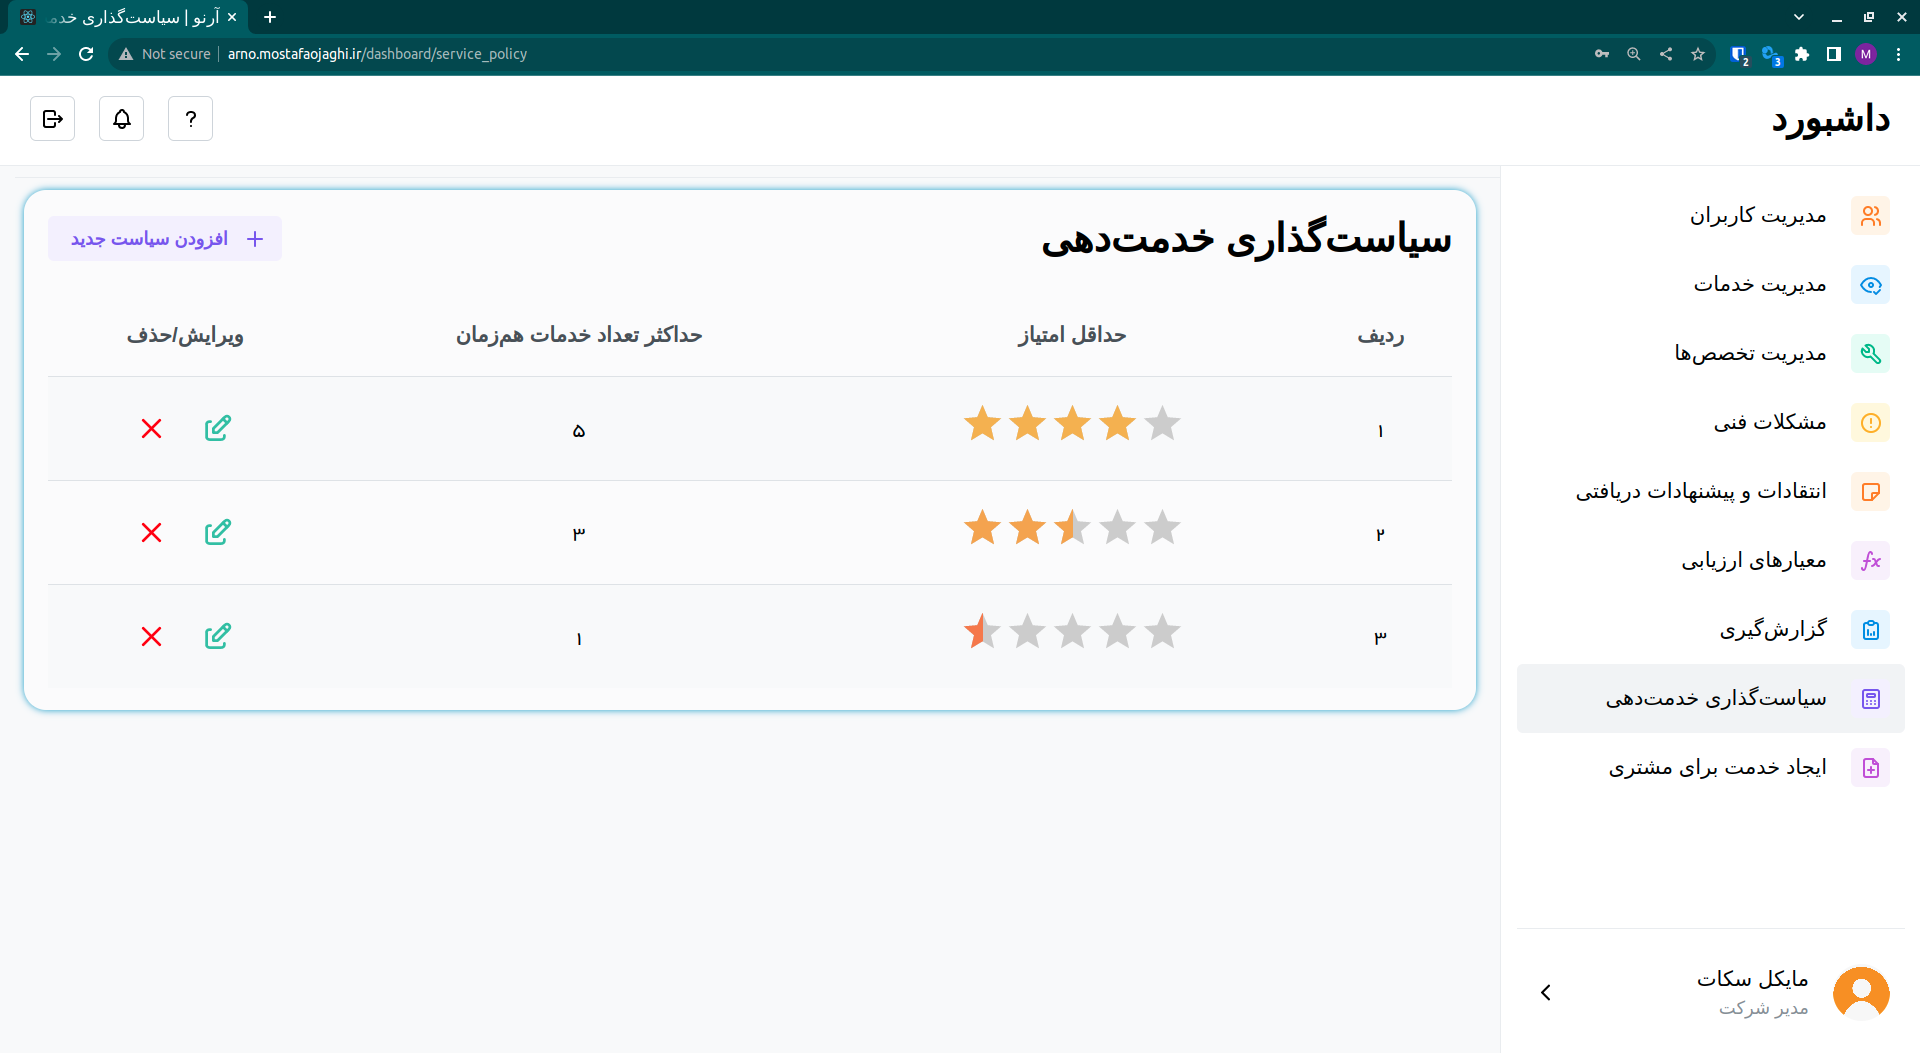
\includegraphics[width=\textwidth]{figs/user-guide/cm-service-policy}
	\caption{صفحه سیاست‌گذاری خدمت‌دهی}
	\label{cm-service-policy}
\end{figure}

\FloatBarrier
